\documentclass[nonacm,acmsmall,screen,11pt]{acmart}

\usepackage{subcaption}

\title{CS4223 Assignment 2: Design and Implementation of Tracing Simulator for MESI, MOESI and Dragon Cache Coherency Protocols}
\author{Julius Putra Tanu Setiaji (A0149787E), Kyle Timothy Ng Chu (A0155181J)}
\makeatletter
\let\@authorsaddresses\@empty
\def\l@subsubsection{\@tocline{3}{0pt}{1pc}{5pc}{}}
\makeatother

\setcounter{tocdepth}{2}

\begin{document}
\maketitle

\tableofcontents

\section{Choice of Programming Language}
Initially, we tried to implement the trace simulator using Python.
However, after a while, we realised that it gets unwieldy, unreadable, and difficult to extend given the complexity of implementing a trace simulator.
Particularly, while Python has enumerations, they are not as powerful as Algebraic Data Types (ADT) in other languages, especially with regards to associated values.
Python's lack of pattern matching also makes implementing a finite state machine (FSM) a hassle.
While Python's dynamic typing allows more rapid prototyping, a better compile-time typecheck would be really useful to prevent bugs.

Haskell seems to fit the bill really well here.
However, since we are essentially simulating a mutable, eagerly-evaluating von Neumann architecture machine, Haskell's characteristic of being immutable and lazy can become an impediment.
We need a language that has some of Haskell's features such as being strongly and statically typed, pattern matching and ADT, while still allowing us to have mutability.
There are some candidates, such as Scala, Rust and OCaml.
For these reasons as well as familiarity, completeness of the standard library and availabilities of third party libraries we chose to implement our tracing simulator using \textbf{Scala}.

\section{Implementation}
Our code can be divided into 2 large parts: common code for all the protocols, and the specific code for the trace simulator of each cache coherency protocols.

Overall, our code uses the delegation pattern, where each device can choose to become a delegate of another device.
This way, devices can have a two-way communication of some sort.
The devices themselves are designed as Finite State Machines (FSM) to allow for more robust code.

There are some potential issues that may prevent correctness in this concurrent system, namely deadlock, livelock, starvation and race conditions \cite{Culler:1998:PCA:2821564}.
As we explain the design of the devices in our simulator, we will mention how we try to prevent these problems from happening.


\subsection{\texttt{Main.scala} and \texttt{Protocol.scala}}
This is the main driver code of the simulator.
It takes in arguments passed by user and parses them into the appropriate types, such as \texttt{Int}, \texttt{String} and \texttt{Protocol}.
\texttt{Protocol} is actually defined inside \texttt{Protocol.scala}, which is an enumeration of supported cache coherency protocols.
In our case we have \texttt{MESI} and \texttt{Dragon}, as well as MOESI for the advanced task.
If all the arguments are parsed successfully, the appropriate tracing simulator is then invoked.

\subsubsection{\texttt{Debug.scala}}
This file provides code for debug printing that can be elided for final production code.

\subsubsection{\texttt{Address.scala}}
This file provides the case class for addressing in an n-way associative cache through tag and set index.

\subsection{\texttt{coherence.bus}}

\subsubsection{\texttt{Bus}}
Across the different protocols, we use the same bus implementation. The design that we chose for our bus is \textbf{an atomic bus}, where one cache is granted exclusive access to the bus to perform one transaction (a transaction is defined as the cache granted exclusive access placing command on the bus, and then receiving response by other caches).

When a device wants to place command on the bus, it has to first request access from the bus, and the device has to be a \texttt{BusDelegate}.
This ensures that a cache will have exclusive access to the bus, with the bus arbitrer acting like a mutex lock.
The bus arbitrer uses a first come first serve arbitration policy to \emph{prevent starvation}.

When the bus arbitrer decides that it is the turn for one \texttt{BusDelegate} to obtain exclusive access to the bus, the bus will invoke \texttt{busAccessGranted()} on the \texttt{BusDelegate} to obtain the command that the device wants to place on the bus.
This is to \emph{prevent race condition}, because the transition of the states of the cache lines are not actually atomic even though the bus is atomic.
Consider the case in MESI protocol when Processors P1 and P2 write to cache line A simultaneously (both need to issue \texttt{BusUpgr} to move the line from the \texttt{S} state to the \texttt{M} state). Suppose P1 wins bus access and places \texttt{BusUpgr} on the bus.
P2 is still waiting for bus access to place its own \texttt{BusUpgr}, but it cannot proceed because P1 has exclusive access to the bus.
P2 then receives \texttt{BusUpgr} from \texttt{P1}, thus it must invalidate line A according to the MESI protocol.
As such, P2 must also change its pending \texttt{BusUpgr} request to a \texttt{BusRdX}.
With our design, we will only ask the cache what command to place on the bus when they are granted access, thus allowing the caches to change the command that they send between the moments access is requested and access is granted.

After a device places a command on the bus, \texttt{onBusCompleteMessage} method on all other devices as \texttt{BusDelegate} will get invoked.
This allows them to make internal state transitions in response to the command on the bus, as well as place their response on the bus.
The bus will arbitrarily grant one device to place their response on the bus.
Once the device having exclusive access to the bus decided that it has received enough responses, it will indicate to the bus that it wishes to relinquish its exclusive access.
This fact is propagated to all other devices through invocation of the \texttt{onBusTransactionEnd} of the \texttt{BusDelegate}.
The bus will then pick another pending access request, and perform the same cycle all over again.
Note that to \emph{avoid livelock}, the device that obtains exclusive access must be allowed to complete before exclusive access is relinquished, thus our design of letting the device decide when to relinquish exclusive access of the bus.
Consider two processors P1 and P2 writing to cache block B using MESI cache coherency protocol.
First, P1 acquired access to the bus and issues \texttt{BusRdX}, resulting in P2 invalidating its cache line.
However, without exclusive ownership, this scenario can happen: before P1 can perform the write, P2 acquires bus, issues \texttt{BusRdX}, resulting in P1 invalidating its cache line, and so on so forth, which results in a livelock.

Note that in our bus design, each device connected to the bus is not blocked on requesting access to the bus.
They are still able to service incoming transactions while waiting to be granted exclusive access to the bus.
This is done to \emph{prevent protocol-level deadlock}, sometimes called \emph{fetch-deadlock} \cite{Culler:1998:PCA:2821564}.

Our bus is implemented as an FSM with 4 states:
\begin{enumerate}
  \item \texttt{Ready} -- no cache has exclusive access to the bus (the mutex lock is not acquired)
  \item \texttt{ProcessingRequest} -- Processing a message from a cache, since only a finite amount of data can be transferred to the bus in a cycle
  \item \texttt{RequestSent} -- A message has been posted on the bus, and the bus is accepting replies from the other devices
  \item \texttt{ProcessingReply} -- Processing a reply from a cache, since only a finite amount of data can be transferred to the bus in a cycle
\end{enumerate}

The state transition can be seen in Figure~\ref{fig:bus}.

\begin{figure}[htb!]
  \centering
  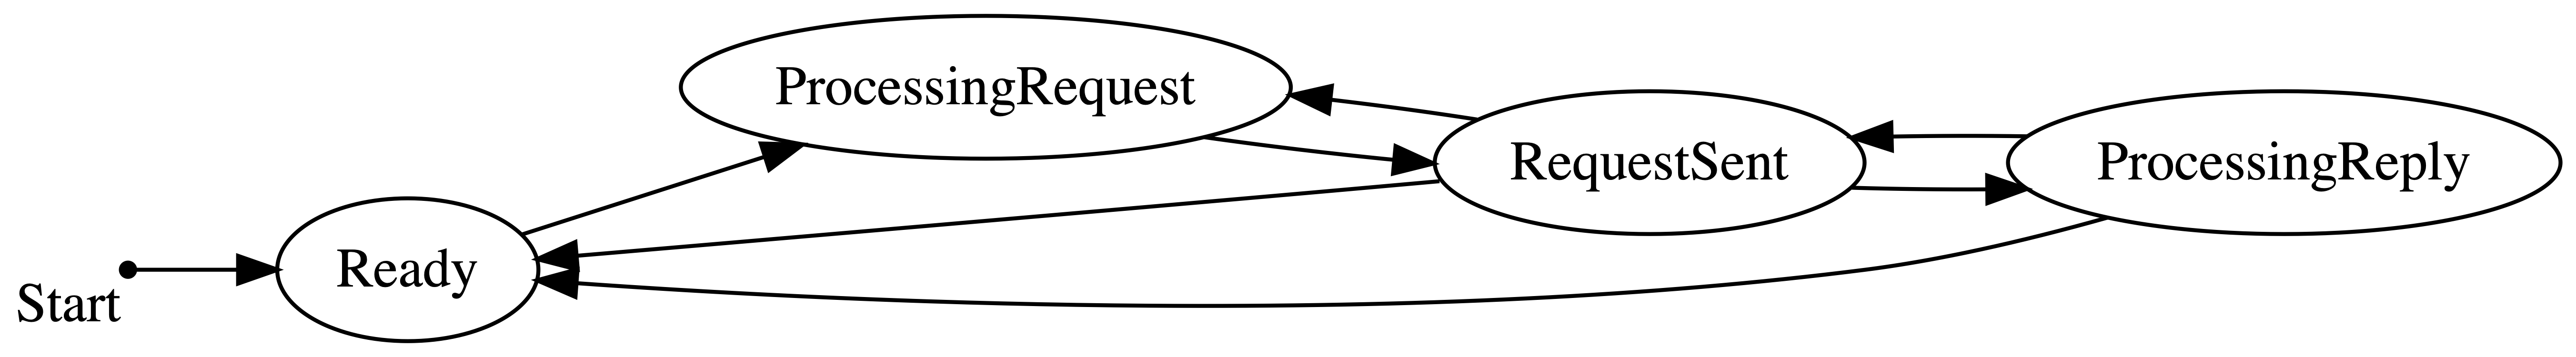
\includegraphics[width=\textwidth]{bus}
  \caption{State Transition for the Bus}
  \label{fig:bus}
\end{figure}

\subsubsection{\texttt{BusDelegate}}
Specifies the hooks in a device that wants to hear back from the \texttt{Bus} regarding events on the Bus.
Of interest is the \texttt{hasCopy} method, which is invoked in order to check the ``SHARED'' OR line, required by the protocols to check whether a particular cache line already exists in the other caches.

\subsubsection{\texttt{BusStatistics}}
This is a ``template'' for each protocol to provide a class that takes note of statistics in the \texttt{Bus}

\subsubsection{\texttt{MessageMetadata}}
A case class that stores the message that a cache wants to place on the bus, as well as the address affected by that message.
The size of each message if not explicitly given is assumed to be 1 byte long.

\subsubsection{\texttt{ReplyMetadata}}
A case class that stores the reply from other caches, as well as the size of the reply.
The size here will be used in the calculation of how long it takes to transmit the reply and associated data on the Bus.

\subsection{\texttt{coherence.cache}}
This package contains classes necessary to build a cache with a Least Recently Used (LRU) cache eviction policy and where each cache line stores a state.

\subsubsection{\texttt{LRUCache}}
This is a simple cache with LRU cache eviction policy that can be used for each set in an n-way associative cache.
It is implemented on top of Java's built-in \texttt{LinkedHashMap} which uses a hash table and linked list to keep track of the order of when an item was last used.

\subsubsection{\texttt{CacheLine}}
This is a simple case class representing a cache line.
It is generic in the type parameter \texttt{State}, and stores only the state of this cache line.

\subsection{\texttt{coherence.devices}}
This package contains mostly the ``template'' for each type of specific devices.
This helps to keep our code DRY\footnote{Don't Repeat Yourself, one important Software Engineering Principle} as the common code among all the protocol are put here.

\subsubsection{\texttt{Device}}
A simple ``template'' for all devices in the simulator.
It only requires that every device has a method \texttt{cycle()} which is invoked to notify the device to advance one cycle and perform what they need to do in a cycle.

\subsubsection{\texttt{Memory}}
This is the ``template'' for a memory in each protocol.
The memory will always return false as it is the identity value in the OR operation on the shared line, thus the memory will not affect the ``SHARED'' OR line.

\subsubsection{\texttt{Processor}}
This is a concrete class that represents a processor in the simulator.
Each processor owns a cache, where the procesor is the cache's \texttt{CacheDelegate}.
It is an FSM with 4 states, with transitions as shown in Figure~\ref{fig:processor}:
\begin{itemize}
  \item \texttt{Ready} -- the processor is ready to execute the next instruction.
  \item \texttt{Operation} -- the processor is currently executing a non-memory instruction
  \item \texttt{Cache} -- the processor is waiting for the result of a memory instruction from its cache
  \item \texttt{Finished} -- the processor has no more instruction to execute
\end{itemize}

\begin{figure}[htb!]
  \centering
  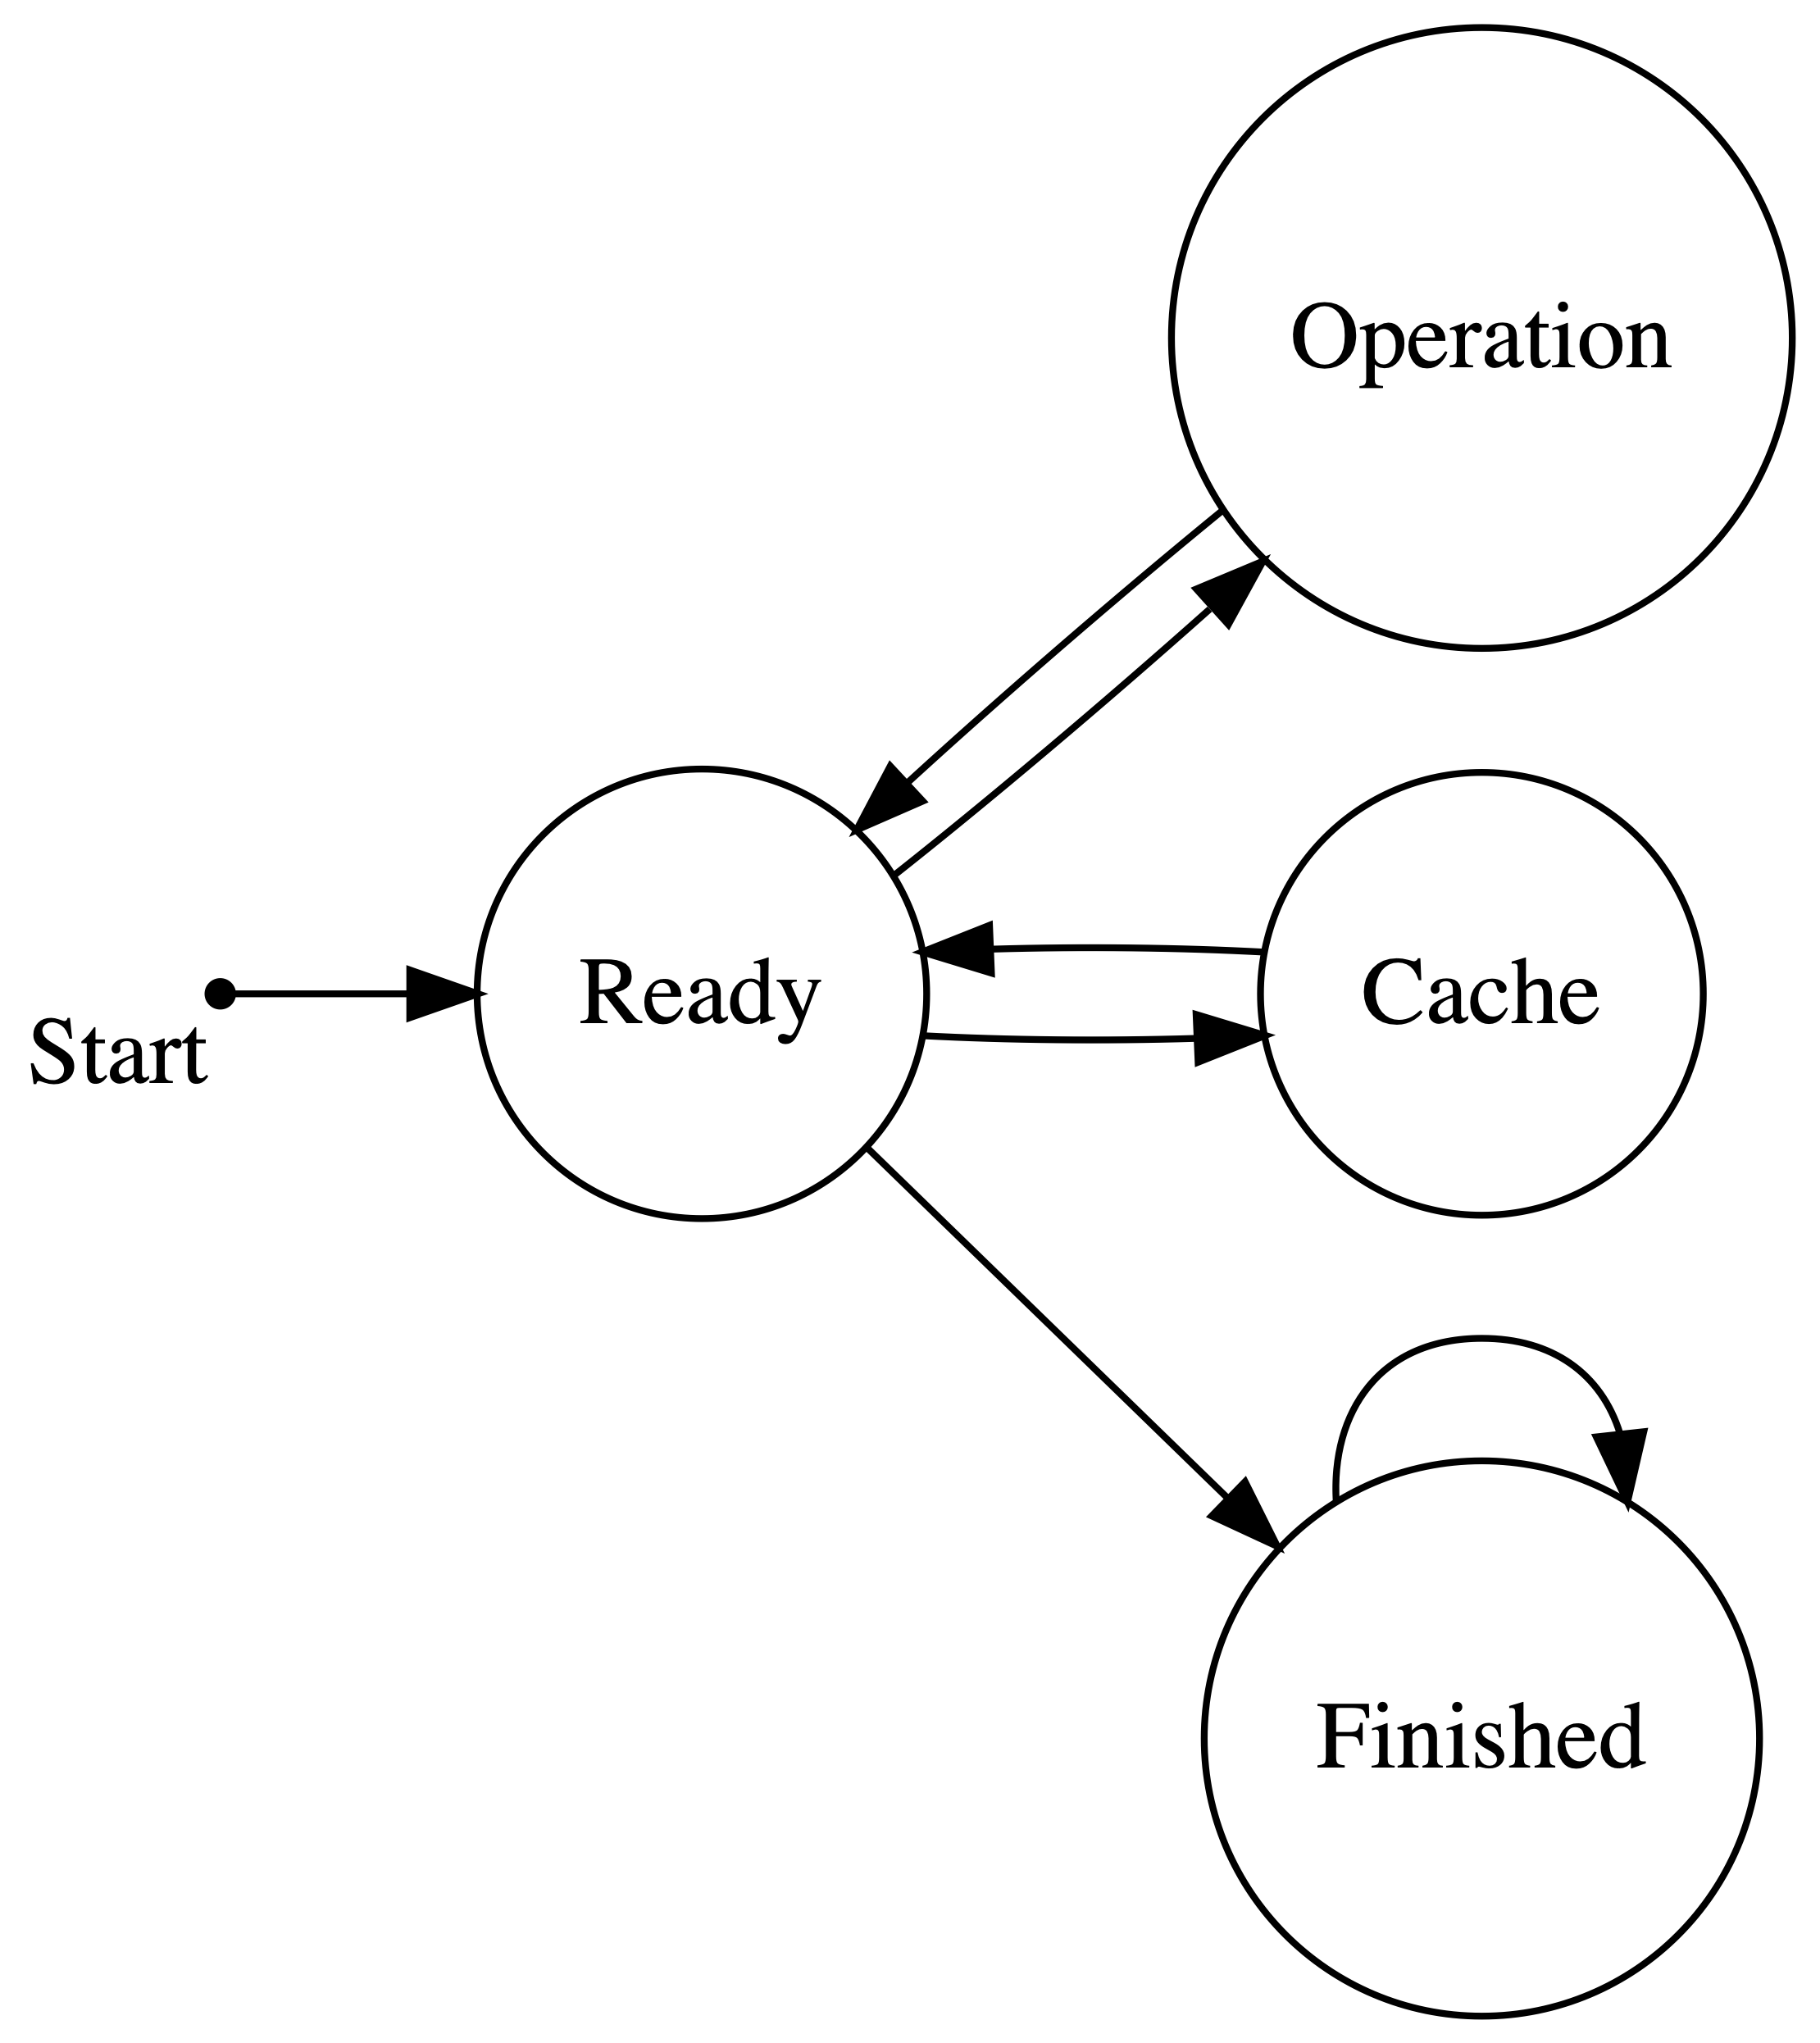
\includegraphics[width=0.3\textwidth]{processor}
  \caption{The state diagram for the processor}
  \label{fig:processor}
\end{figure}

\subsubsection{\texttt{ProcessorOp}}
This trait is effectively an ADT representing the three possible instructions: the memory instructions \texttt{Load} and \texttt{Store} which has the address as the associated value as well as the non-memory instruction \texttt{Other} with the number of cycles required for execution as the associated value.
The associated singleton object of the \texttt{ProcessorOp} trait provides a function to parse each line in the input trace into a \texttt{ProcessorOp}.

\subsubsection{\texttt{Cache}}
This is the ``template'' for the protocol-specific implementation of the cache.
The cache is an FSM with 8 states, whereby each state will inform the cache about what to do with regards to the bus:
\begin{itemize}
  \item \texttt{Ready} -- the cache is ready to accept commands from the processor
  \item \texttt{WaitingForBus} -- the cache has requested access to the bus but is waiting for that access to be granted
  \item \texttt{WaitingForReplies} -- the cache has exclusive access to the bus and has placed a message on the bus, and is waiting for replies from the other caches.
  \item \texttt{WaitingForWriteback} -- the cache has exclusive access to the bus and has snooped a Flush request, and is currently waiting for the memory to acknowledge that the writeback succeeded.
  \item \texttt{WaitingForResult} -- the cache has the cache line requested, and that cache line is valid, and the cache is currently experiencing its hit latency.
  \item \texttt{WaitingForBusPropagation} -- the cache sent a message on the bus and is waiting for the message to reach the other caches.
  \item \texttt{EvictWaitingForBus} -- the cache needs to evict a cache line, has requested access to the bus and is currently waiting for that access to be granted.
  \item \texttt{EvictWaitingForWriteback} -- the cache currently has exclusive access to the bus and has placed the flush command on the bus and is waiting for the memory to acknowledge the writeback.
\end{itemize}

The state transitions are shown in Figure~\ref{fig:cache}

\begin{figure}[htb!]
  \centering
  
\includegraphics[width=\textwidth]{cache}
  \caption{The state diagram for the cache}
  \label{fig:cache}
\end{figure}

\subsubsection{\texttt{CacheDelegate}}
This is the ``template'' for a cache delegate, which requires only one method, \texttt{requestCompleted} which is invoked when the operation is complete.

\subsubsection{\texttt{CacheOp}}
An ADT representing the possible cache operations.

\subsubsection{\texttt{CacheStatistics}}
This is a ``template'' for each protocol to provide a class that takes note of statistics in the \texttt{Cache}

\subsection{MESI Protocol (\texttt{coherence.mesi})}
The MESI protocol consists of four states: Modified (M), Exclusive (E), Shared (S), and Invalid (I).
The state transition diagram can be found in Figure~\ref{fig:mesi}.
For any given pair of caches, the permitted states of a given cache line is given in Table~\ref{tab:mesi}

\begin{figure}[htb!]
  \centering
  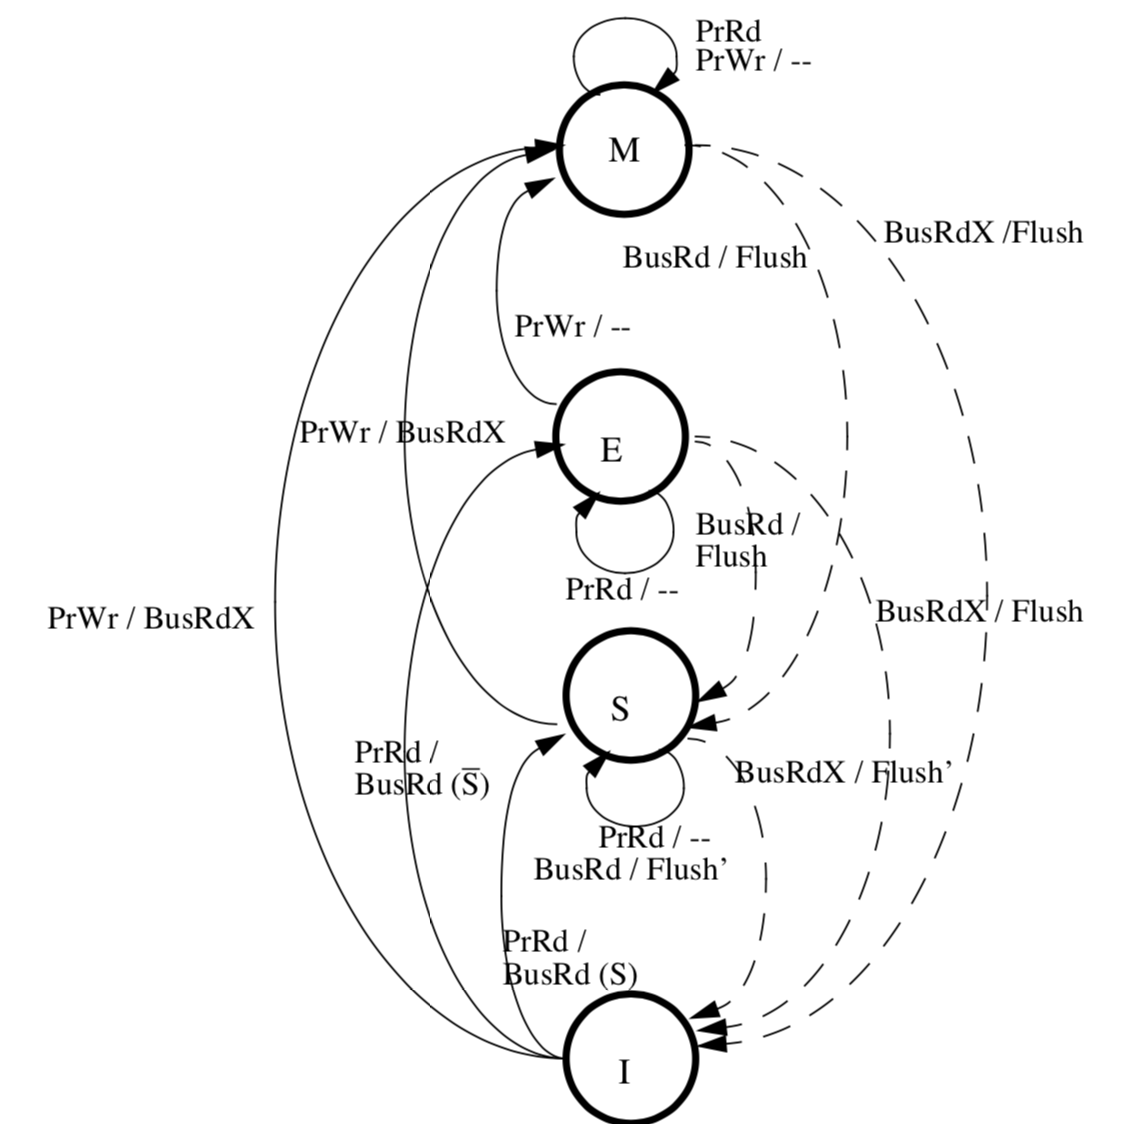
\includegraphics[width=0.5\textwidth]{mesi}
  \caption{State Transition Diagram of the MESI Cache Coherency Protocol}
  \label{fig:mesi}
\end{figure}

\begin{table}[htb!]
  \centering
  \caption{Permitted States for a Pair of Caches in MESI Protocol}
  \label{tab:mesi}
  \begin{tabular}{|l|l|l|l|l|}
    \hline
               & \textbf{M} & \textbf{E} & \textbf{S} & \textbf{I} \\ \hline
    \textbf{M} & No         & No         & No         & Yes        \\ \hline
    \textbf{E} & No         & No         & No         & Yes        \\ \hline
    \textbf{S} & No         & No         & Yes        & Yes        \\ \hline
    \textbf{I} & Yes        & Yes        & Yes        & Yes        \\ \hline
  \end{tabular}
\end{table}

\subsubsection{Message}
There are 4 possible messages to be placed by a cache that gained exclusive access to the bus:
\begin{enumerate}
  \item \texttt{BusRd} -- a read request to a cache block
  \item \texttt{BusRdX} -- a read exclusive request to a cache block, typically when a cache wants to write to a cache block it does not already have.
  \item \texttt{BusUpgr} -- a request to gain read exclusive access to a shared cache block that a cache already has.
  \item \texttt{Flush} -- a request to write back the cache block to the main memory
\end{enumerate}

\subsubsection{Reply}
There are 4 possible replies to be placed by a cache or memory to a Message:
\begin{enumerate}
  \item \texttt{Flush} -- when a cache block must be written back to the main memory
  \item \texttt{FlushOpt} -- when a cache block is posted on the bus to supply it to another cache
  \item \texttt{MemoryRead} -- when the memory posts a cache block on the bus
  \item \texttt{WritebackOk} -- acknowledgement from the memory that a cache block has been written successfully
\end{enumerate}

\subsubsection{Memory}
The memory in our MESI Protocol simulator snoops on the bus and will do one of these three things:
\begin{enumerate}
  \item Do nothing if the command is \texttt{BusUpgr}
  \item Read from the address in the command placed by a cache if the command is \texttt{BusRd} or \texttt{BusRdX}
  \item Write back to memory if the command is \texttt{Flush}
\end{enumerate}

If the memory detects that another cache is providing the cache line instead, e.g. if the state is S, then the memory will cancel the current read request.
If the memory detects that a cache replied with OK, it will cancel the read request, and start the writeback process instead.

\subsubsection{Cache}
This is the specific implementation of abstract class \texttt{Cache} from \texttt{coherence.devices} for the MESI protocol according to the state transition diagram in Figure~\ref{fig:mesi}

In our implementation, in case of cache line that is shared, the one supplying the block will be arbitrarily picked, depending on the one that was able to place its reply on the bus first.
When other caches detect that the block content has been posted on the bus, they will change state so as to not double-send the block.

\subsection{MOESI Protocol (\texttt{coherence.moesi}): Optimisation to Basic MESI Protocol}
Some processor architectures such as UltraSPARC \cite{microelectronics1997ultrasparc} and AMD Opteron \cite{Jacob:2007:MSC:1543376} use an optimised version of the MESI protocol by adding one more state: O for Owned, representing a cache line that is both modified and shared.
The idea is to allow cache having a modified cache line to supply that data to another cache without performing a slow writeback to memory.
The state transition diagram can be found in Figure~\ref{fig:moesi}. For any given pair of caches, the permitted states of a given cache line is given in Table~\ref{tab:moesi}.

\subsubsection{Differences Compared to MESI}


\begin{figure}[htb!]
  \centering
  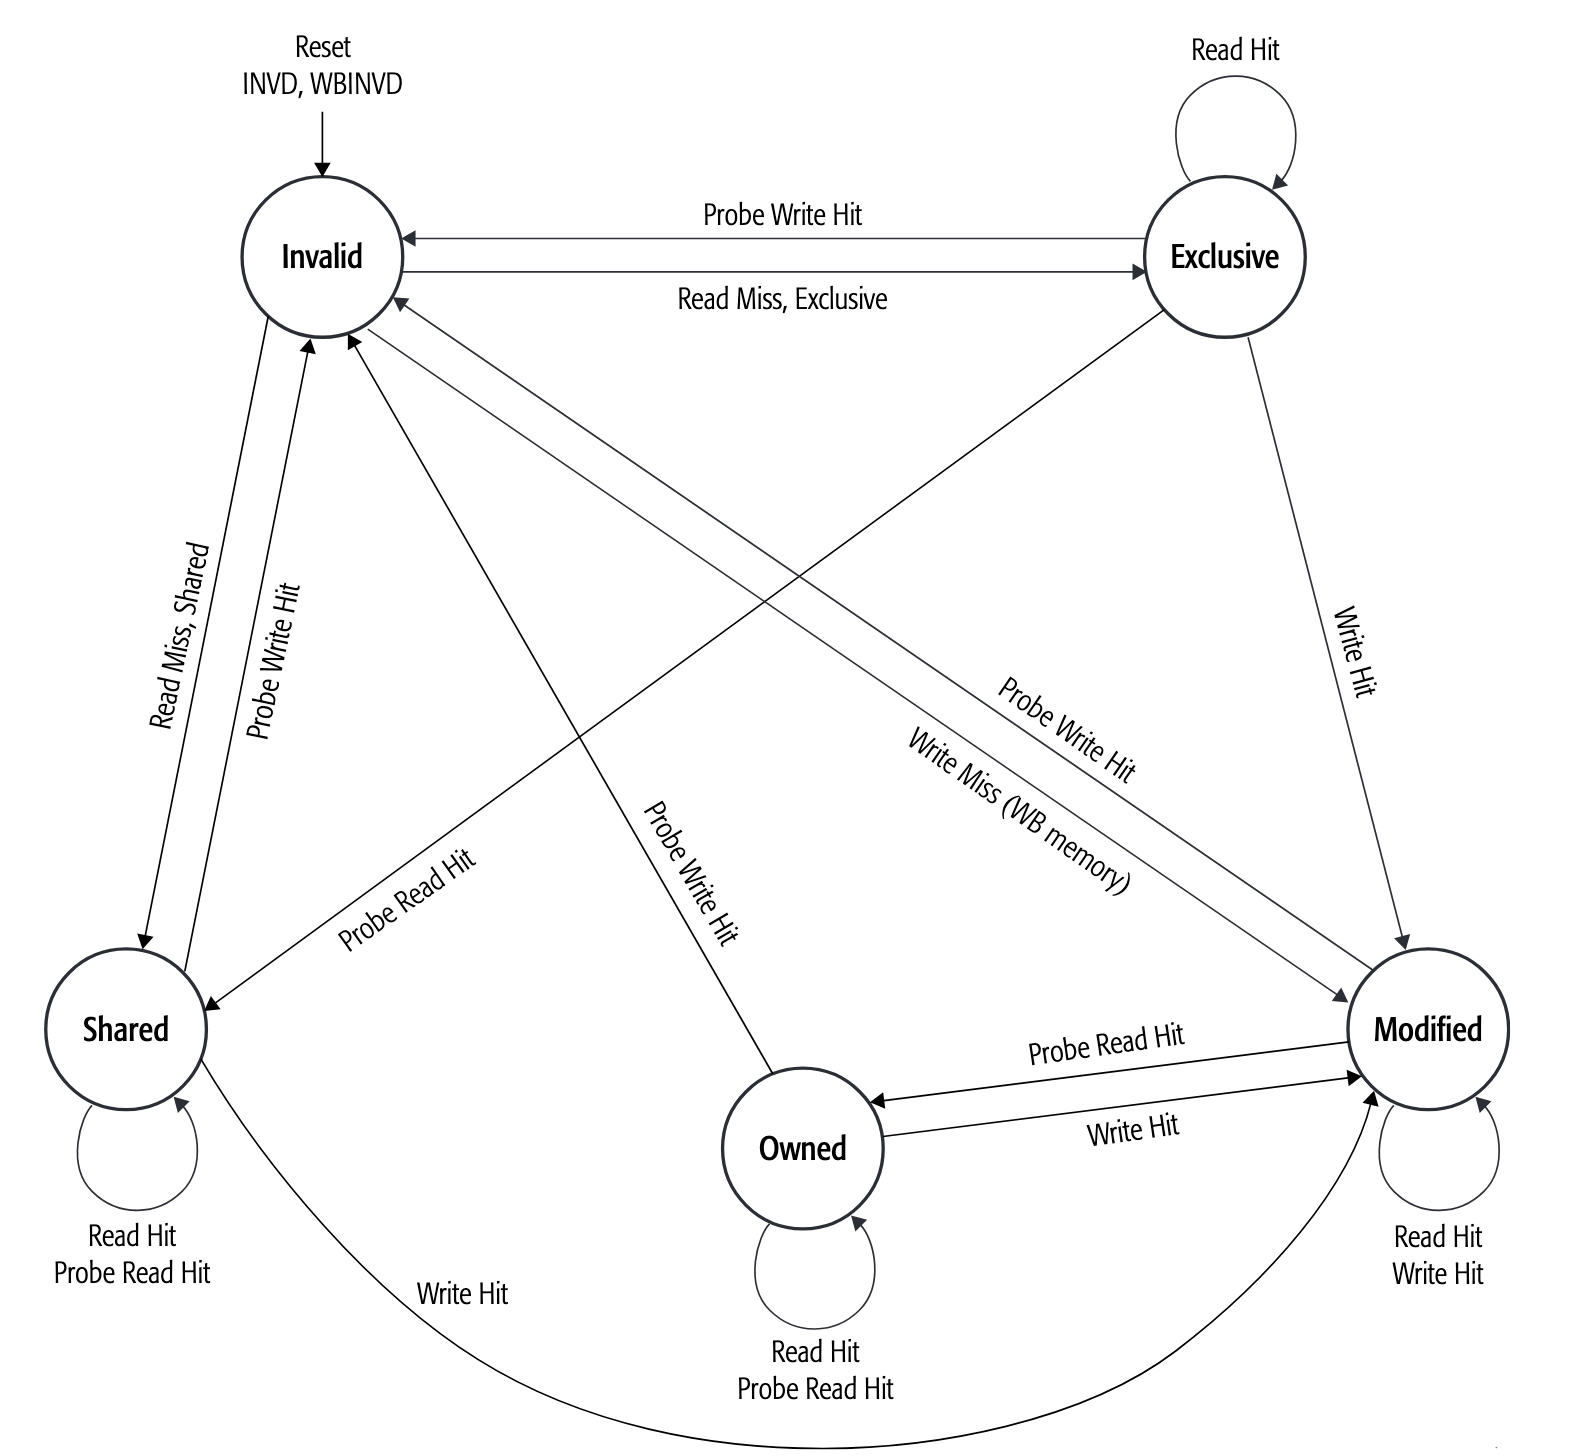
\includegraphics[width=0.7\textwidth]{moesi}
  \caption{State Transition Diagram of the MOESI Cache Coherency Protocol}
  \label{fig:moesi}
\end{figure}

\begin{table}[htb!]
  \centering
  \caption{Permitted States for a Pair of Caches in MESI Protocol}
  \label{tab:moesi}
  \begin{tabular}{|l|l|l|l|l|l|}
    \hline
               & \textbf{M} & \textbf{O} & \textbf{E} & \textbf{S} & \textbf{I} \\ \hline
    \textbf{M} & No         & No         & No         & No         & Yes        \\ \hline
    \textbf{O} & No         & No         & No         & Yes        & Yes        \\ \hline
    \textbf{E} & No         & No         & No         & No         & Yes        \\ \hline
    \textbf{S} & No         & Yes        & No         & Yes        & Yes        \\ \hline
    \textbf{I} & Yes        & Yes        & Yes        & Yes        & Yes        \\ \hline
  \end{tabular}
\end{table}

\subsection{Dragon Protocol}
The Dragon Protocol is a write-update based cache coherence protocol that was first introduced along with the Dragon Multi-processor \cite{atkinson1987dragon}. Unlike write-invalidate protocols like MESI, Dragon updates shared cache lines at each write instead of just invalidating them. 

\begin{figure}[!htb]
  \centering
  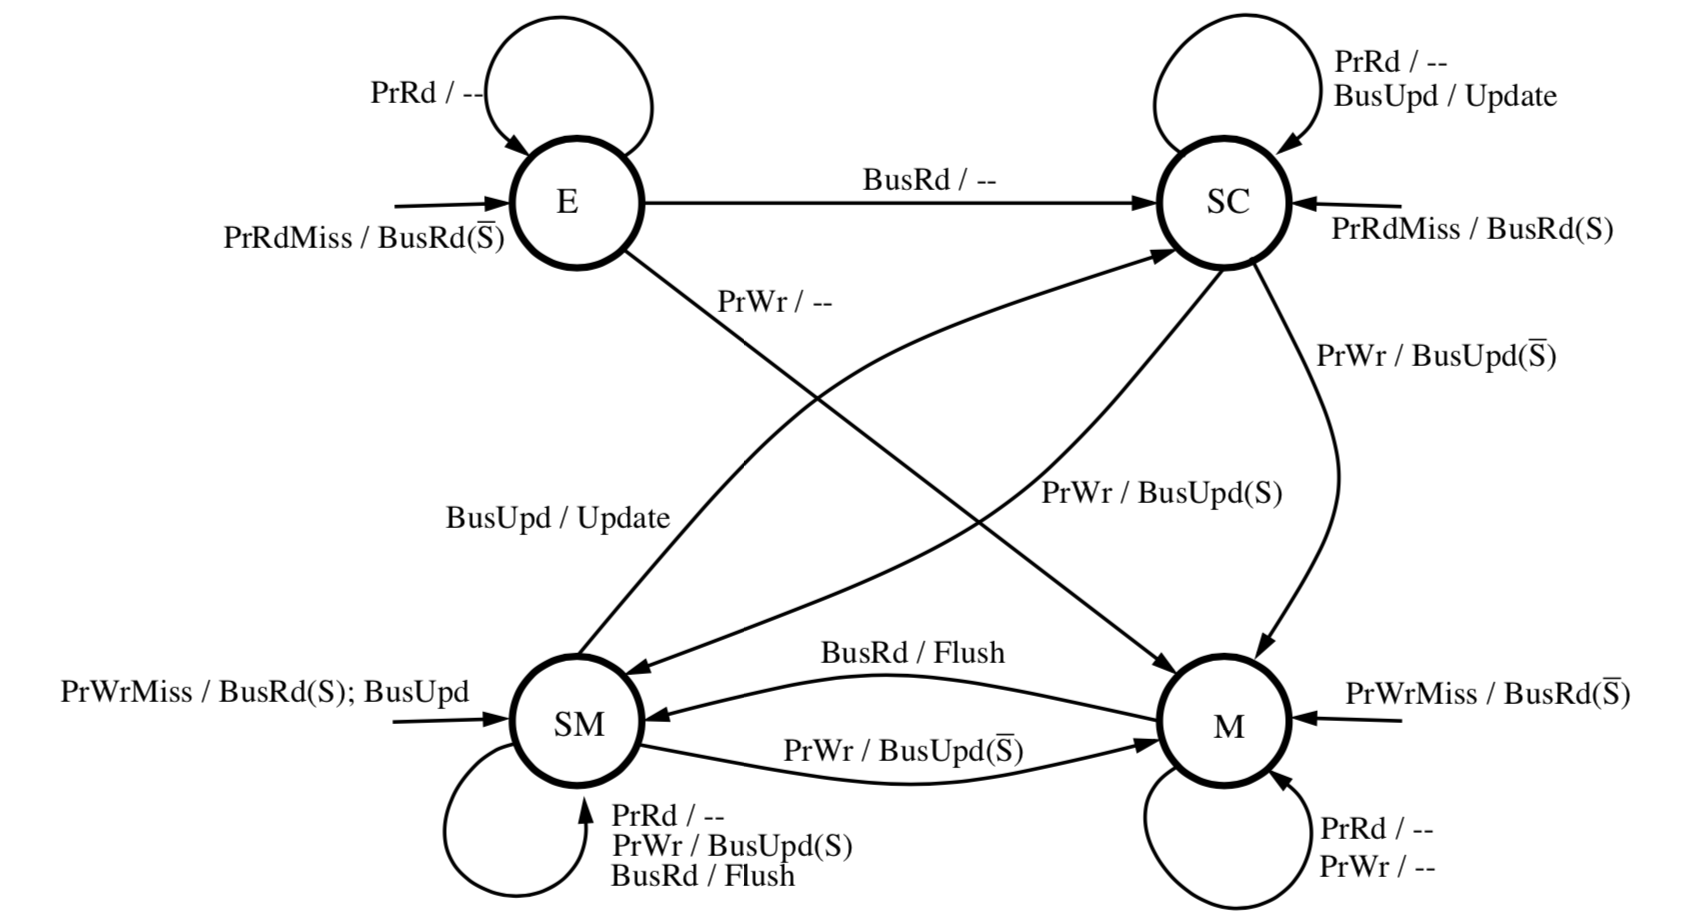
\includegraphics[width=0.8\textwidth]{dragon}
  \caption{State Diagram for the Dragon Protocol}
\end{figure}

\begin{table}[!htb]
  \centering
  \caption{Permitted States for a Pair of Caches in Dragon Protocol}
  \label{tab:dragon}
  \begin{tabular}{|l|l|l|l|l|}
    \hline
                & \textbf{E} & \textbf{Sc} & \textbf{Sm} & \textbf{M} \\ \hline
    \textbf{E}  & No         & No          & No          & No         \\ \hline
    \textbf{Sc} & No         & Yes         & Yes         & No         \\ \hline
    \textbf{Sm} & No         & Yes         & No          & No         \\ \hline
    \textbf{M}  & No         & No          & No          & No         \\ \hline
  \end{tabular}
\end{table}

\subsubsection{Message}
There are 3 possible messages to be placed by a cache that gained exclusive access to the bus:
\begin{enumerate}
  \item \texttt{BusRd} -- a read request to a cache block
  \item \texttt{BusUpt} -- a request to caches that contain the same cache block to update their local copies
  \item \texttt{Flush} -- a request to write back the cache block to the main memory
\end{enumerate}

\subsubsection{Reply}
There are 4 possible replies to be placed by a cache or memory to a Message:
\begin{enumerate}
  \item \texttt{Flush} -- when a cache block must be written back to the main memory
  \item \texttt{MemoryRead} -- when the memory posts a cache block on the bus
  \item \texttt{WritebackOk} -- acknowledgement from the memory that a cache block has been written successfully
\end{enumerate}

\subsubsection{Memory}
The memory in our Dragon Protocol simulator snoops on the bus and will do one of these three things:
\begin{enumerate}
  \item Do nothing if the command is \texttt{BusUpt}
  \item Read from the address in the command placed by a cache if the command is \texttt{BusRd} or \texttt{BusRdX}
  \item Write back to memory if the command is \texttt{Flush}
\end{enumerate}

\clearpage
\section{Quantitative Analysis}
\subsection{Workload Analysis}
Before analysing the results of our simulations, it is important to first briefly analyse the nature of the workloads we used in these experiments. The workloads used are from the PARSEC benchmark suite which is used for benchmarking the performance of multi-core processors \cite{bienia2008parsec}. The table below provides a summary of the key characteristics of the benchmarks.
\begin{table}[!htb]
    \centering
    \label{tab:benchmarks}
    \begin{tabular}{|c|c|c|c|l}
        \cline{1-4}
        \multicolumn{1}{|l|}{\textbf{Benchmark}} & \multicolumn{1}{l|}{\textbf{Granularity}} & \multicolumn{1}{l|}{\textbf{Data Sharing}} & \multicolumn{1}{l|}{\textbf{Data Exchange}} &  \\ \cline{1-4}
        \textit{blackscholes} & Coarse & low & low &  \\ \cline{1-4}
        \textit{bodytrack} & Medium & high & medium &  \\ \cline{1-4}
        \textit{fluidanimate} & Fine & low & medium &  \\ \cline{1-4}
    \end{tabular}
    \caption{Key characteristics of the benchmarks as taken from\cite{bienia2008parsec}}
\end{table}
\begin{itemize}
    \item \textit{blackscholes} - This benchmark consists of a main thread which spawns several worker threads that act on independent sections of data. As a result the majority of shared memory among the threads is between the main thread and the worker threads. Since the worker threads process data independently of each other, there is little communication between the threads.
    \item \textit{bodytrack} - This benchmark has multiple threads working on the same set of data. 
    \item \textit{fluidanimate} - This benchmark has multiple threads working on the same set of data. Due to the nature of the workload, there is a significant amount of inter-thread communication which scales with the number of threads \cite{bienia2008parsec}
\end{itemize}

\subsection{Experimental Results \& Analysis}
We ran our simulations with varying cache sizes, block sizes and set associativity. The results are presented and discussed in the sections below:
\subsubsection{Cache size}
\begin{figure}[htb!]
  \centering
  \begin{subfigure}{0.32\textwidth}
    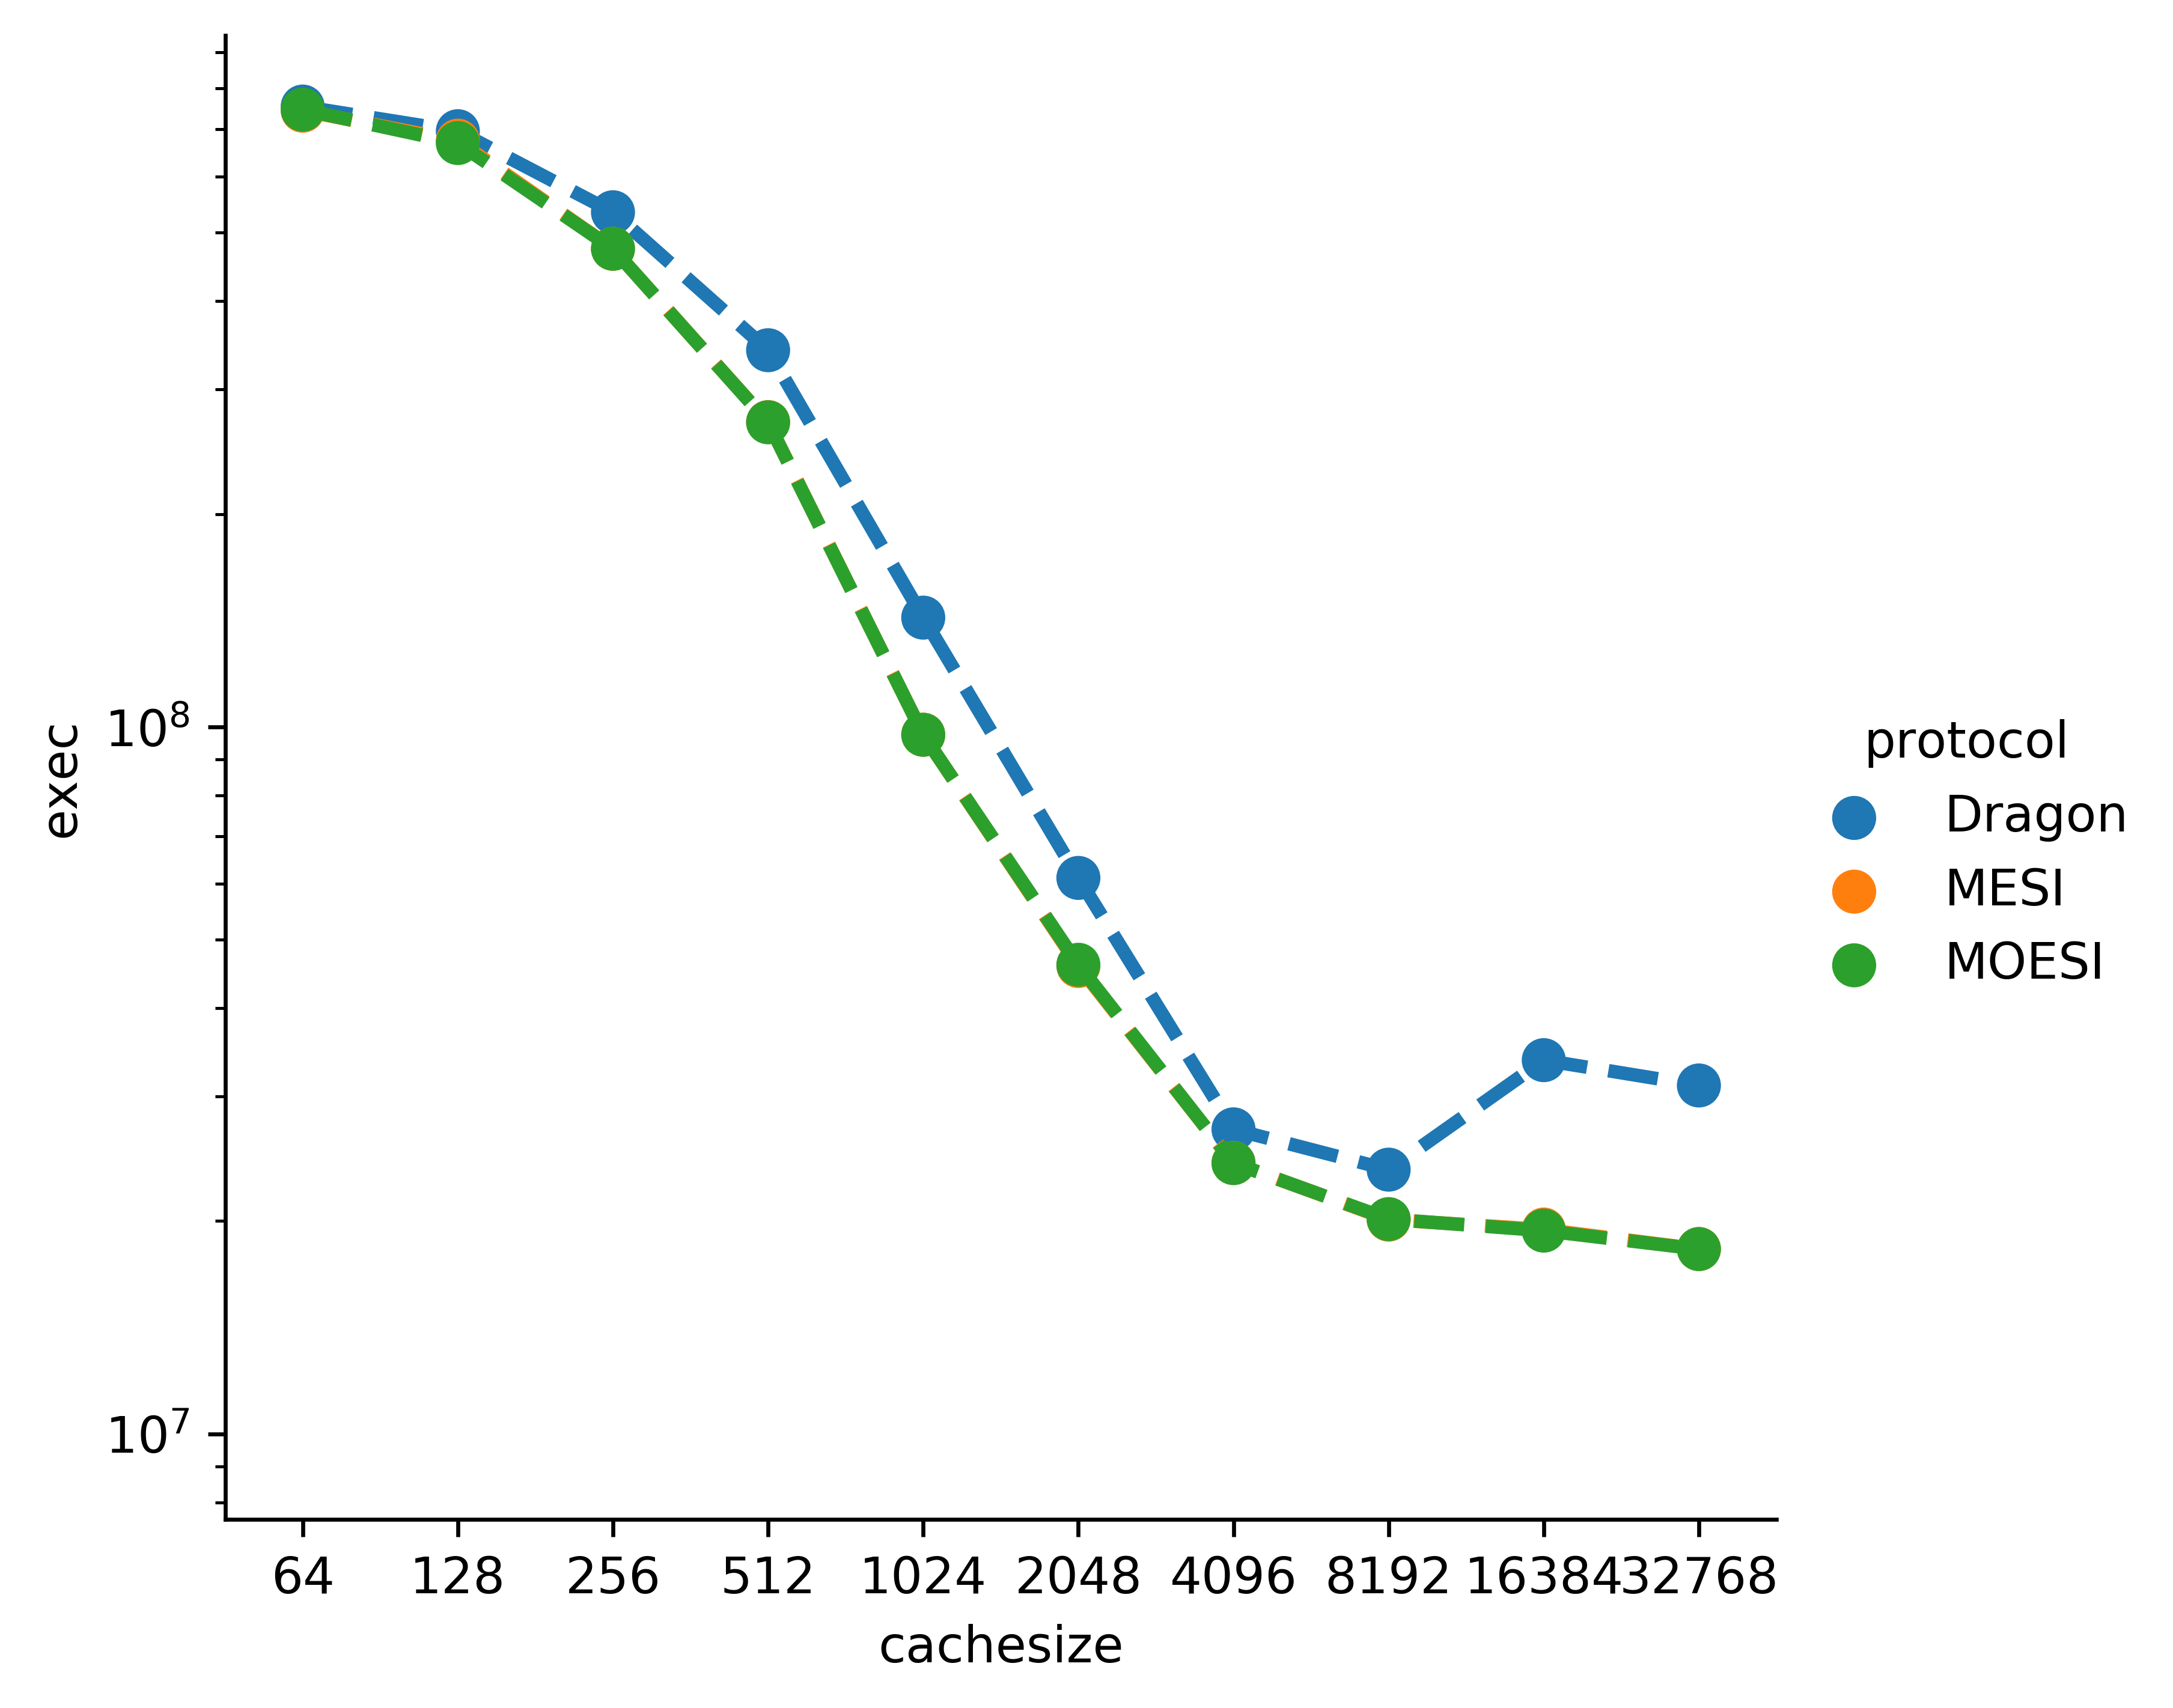
\includegraphics[width=\textwidth]{cachesize-blackscholes}
    \caption{blackscholes}
  \end{subfigure}
  \begin{subfigure}{0.32\textwidth}
    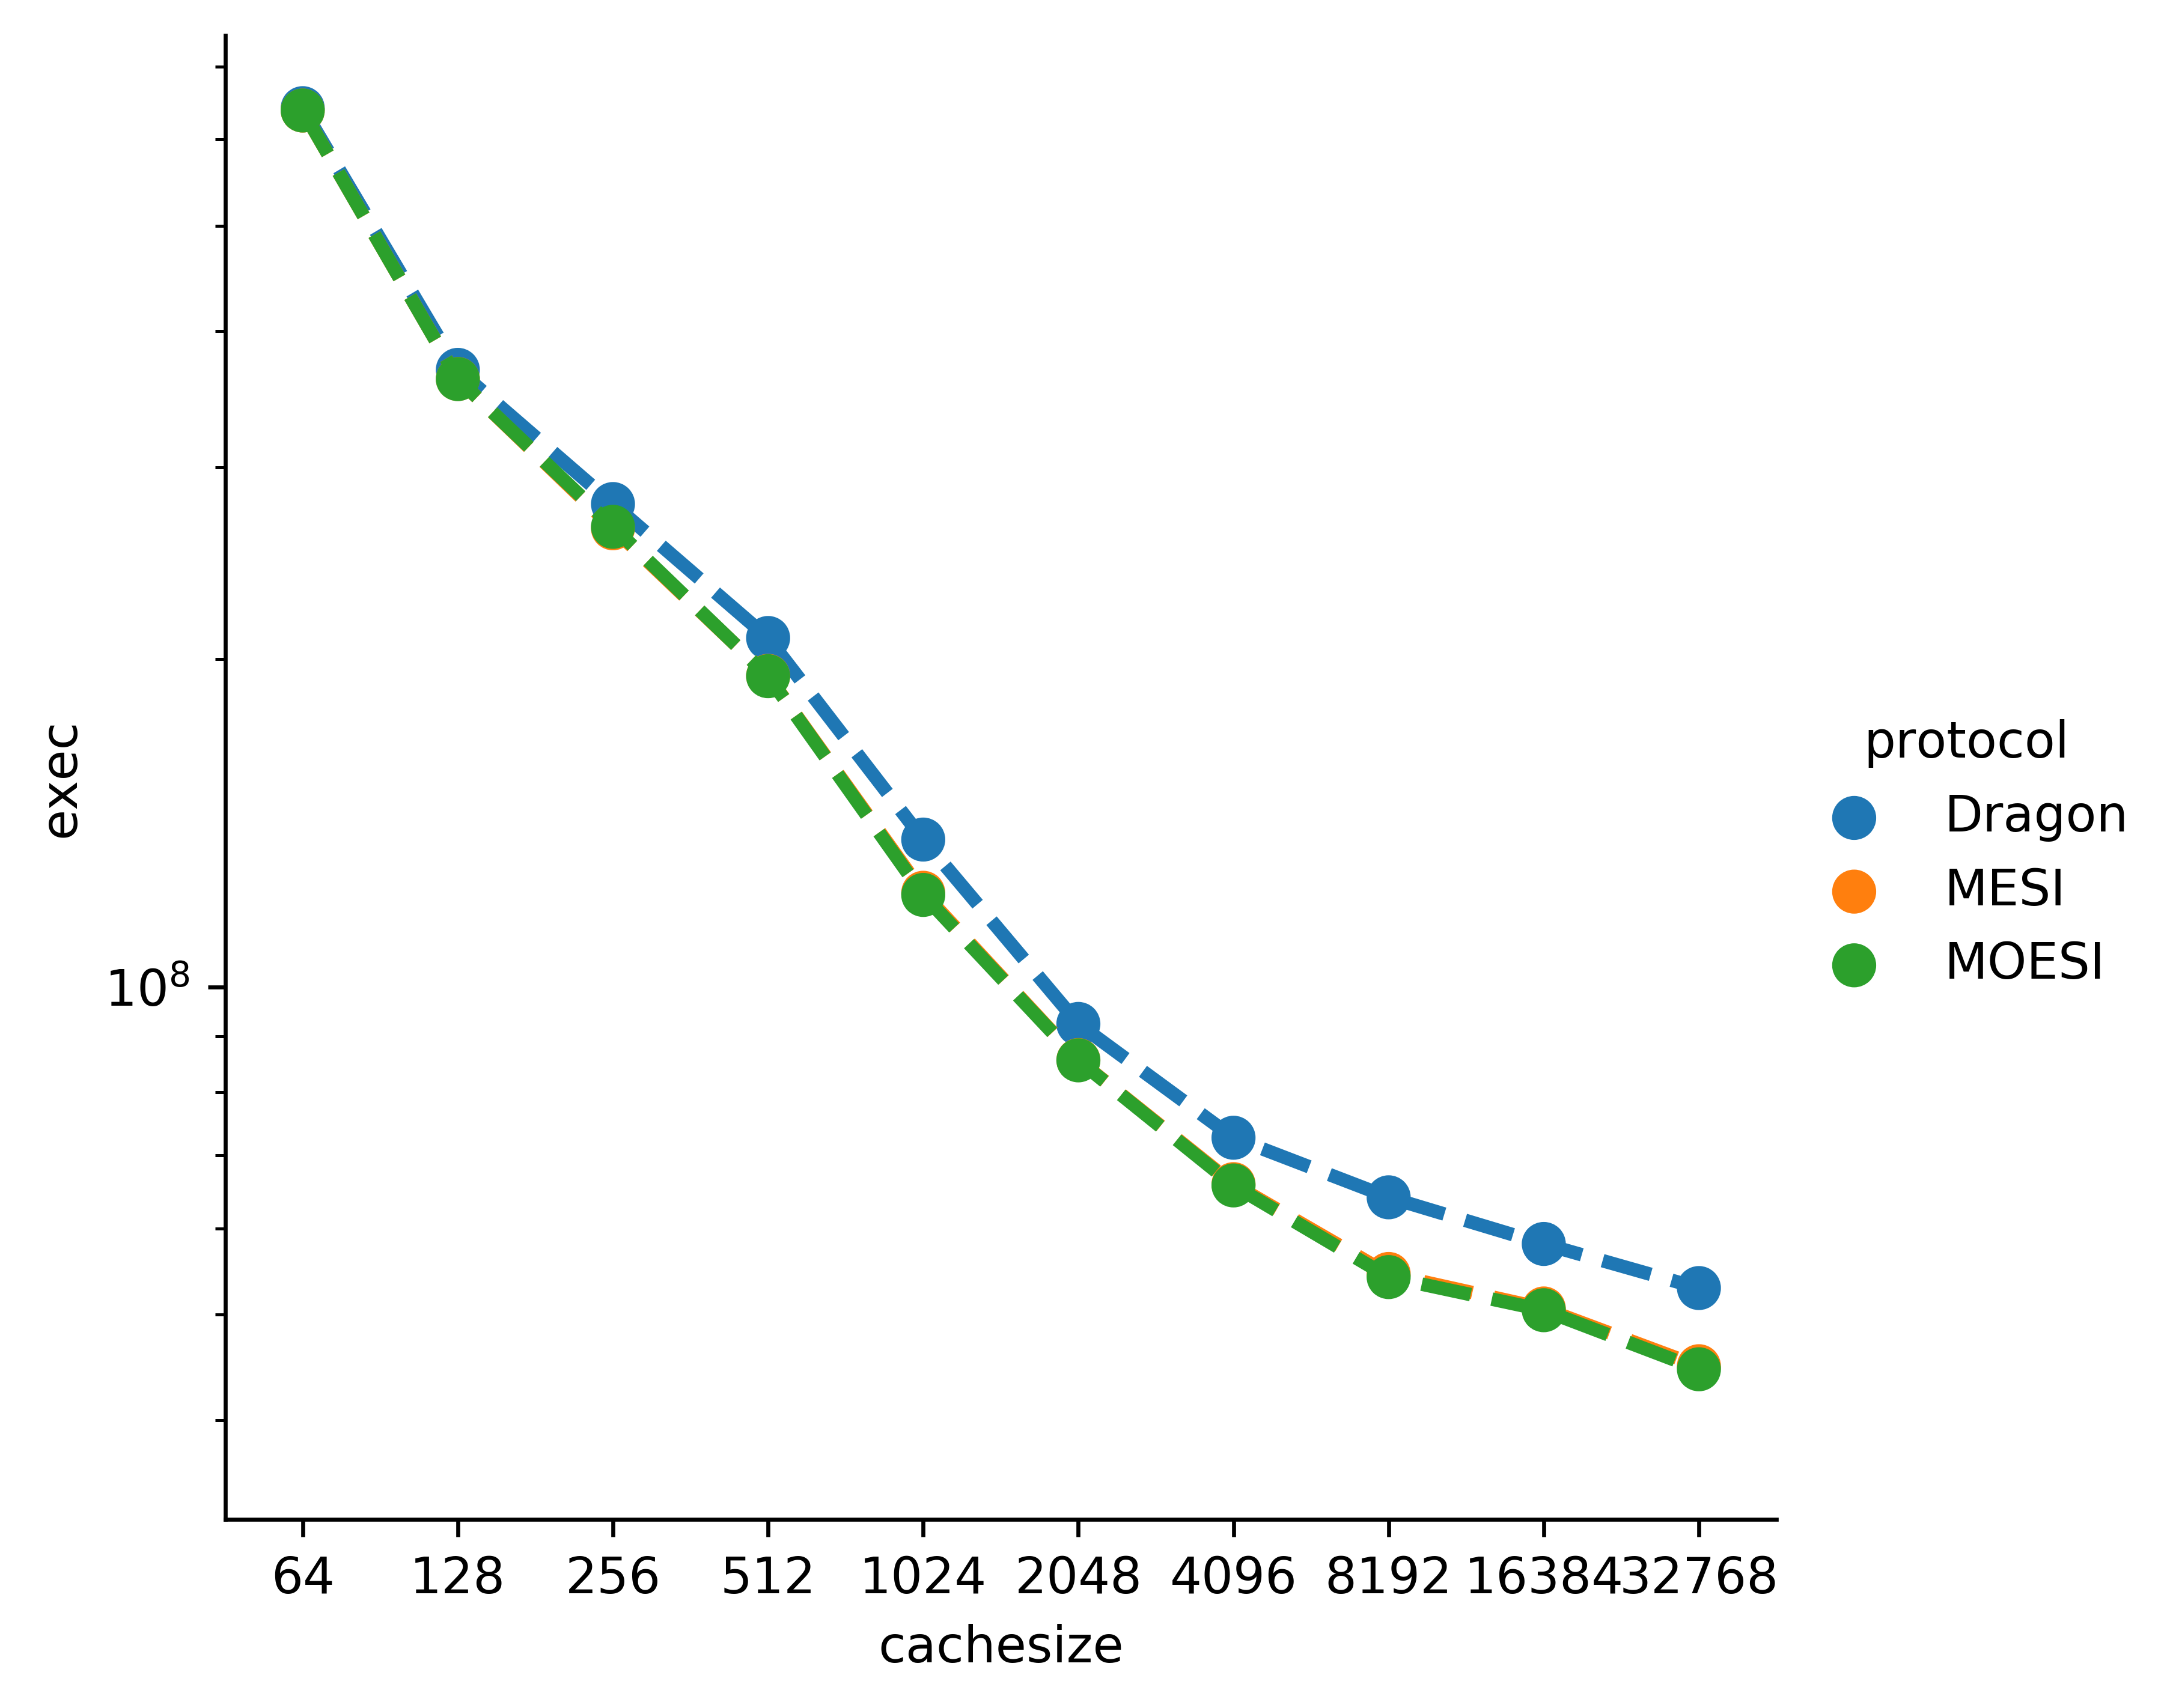
\includegraphics[width=\columnwidth]{cachesize-bodytrack}
    \caption{bodytrack}
  \end{subfigure}
  \begin{subfigure}{0.32\textwidth}
    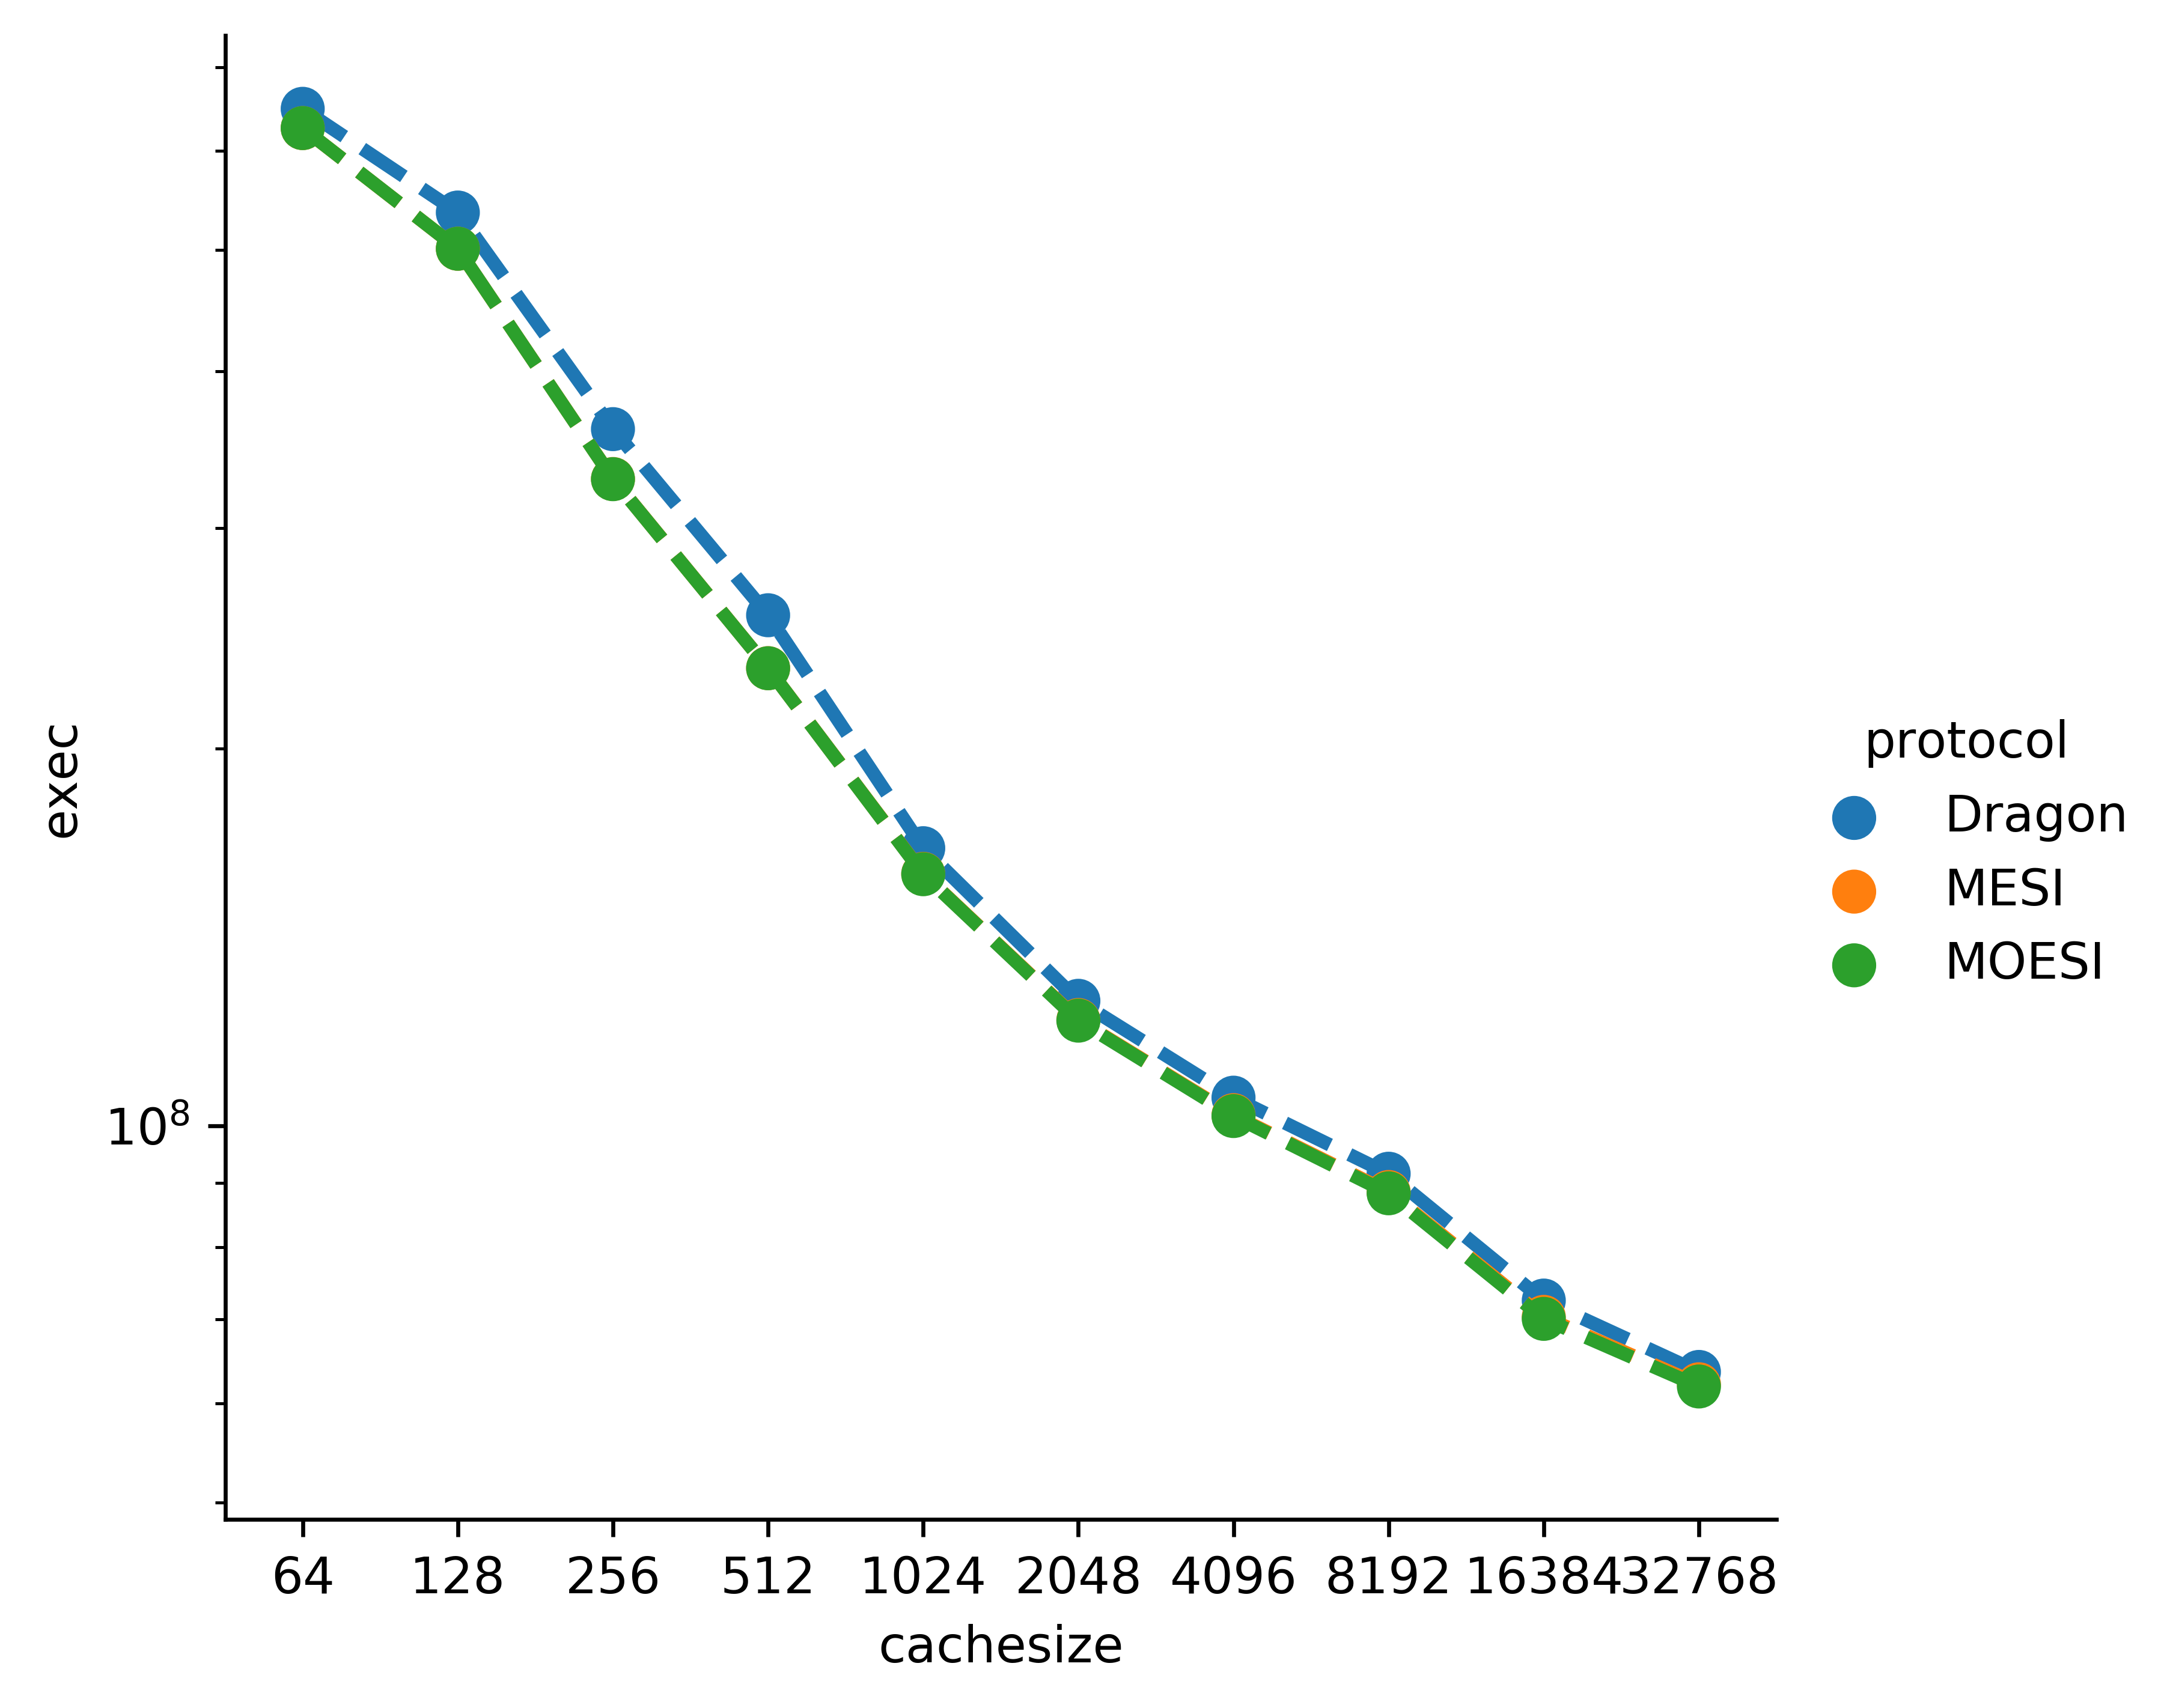
\includegraphics[width=\columnwidth]{cachesize-fluidanimate}
    \caption{fluidanimate}
  \end{subfigure}
  \caption{Plot of total execution cycles against cache size with 2-way associative cache with 32 bytes block size, Note that the line for the MESI protocols may be difficult to see as it almost completely overlaps with the MOESI protocol.}
  \label{fig:cachesize}
\end{figure}
As seen in Figure \ref{fig:cachesize} above, the MOESI/MESI protocol outperforms the Dragon protocol in all 3 benchmarks regardless of cache size. We believe that the reason for this is due to the unnecessary write updates on cache lines that are not read again after they were first cached. This is especially apparent in the \textit{blackscholes} benchmark there is little shared memory. This problem is exacerbated as the cache size increases due to more of such entries remaining in the cache for longer periods of time before they are evicted. We can observe this effect in the \textit{blackscholes} benchmark where the penalty of these unnecessary updates is dominant over the benefit gained from a larger cache size past 8kB. This causes the number of cycles taken to execute the application to increase after that point.
The \textit{fluidanimate} shows much more promising results for the Dragon protocol since there is a high amount of inter-thread communication in the workload. However, we observe that the MOESI/MESI protocol still performs slightly better. One reason for this could potentially attributed to multiple sequential write instructions being executed before a read takes place which is also another source of unnecessary write updates. 

\subsubsection{Block size}
\begin{figure}[htb!]
  \centering
  \begin{subfigure}{0.32\textwidth}
    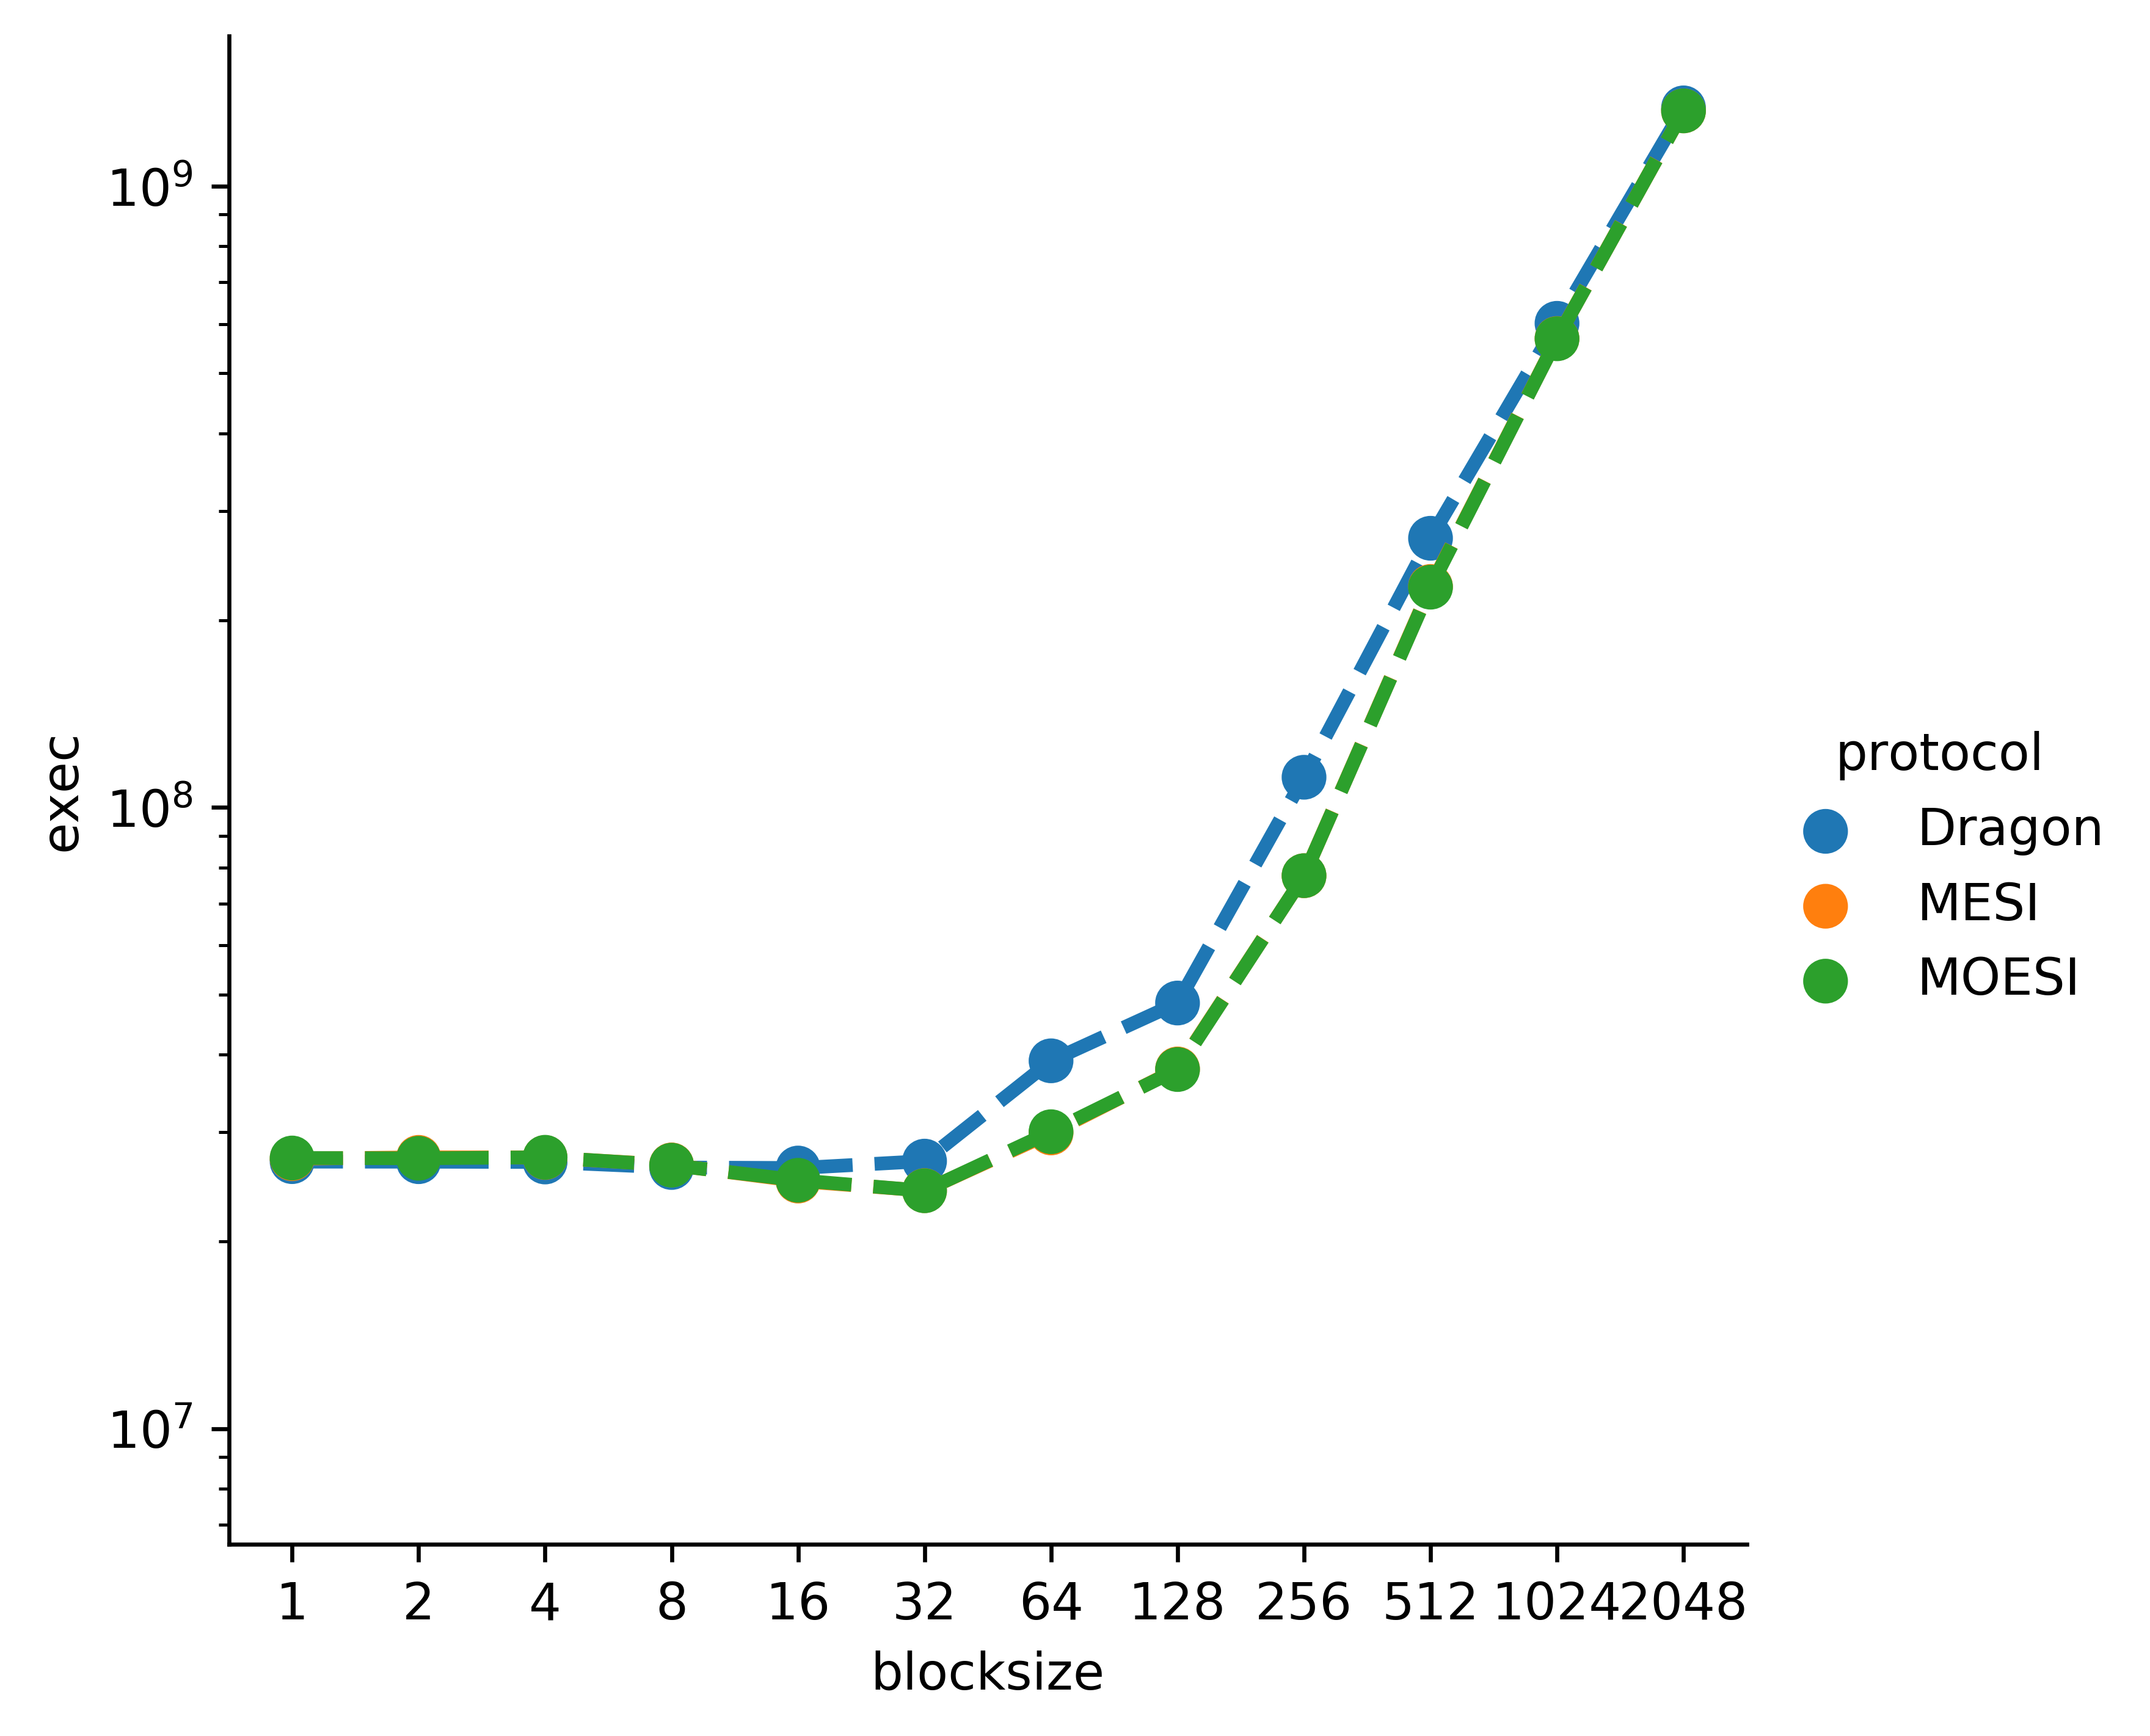
\includegraphics[width=\textwidth]{blocksize-blackscholes}
    \caption{blackscholes}
  \end{subfigure}
  \begin{subfigure}{0.32\textwidth}
    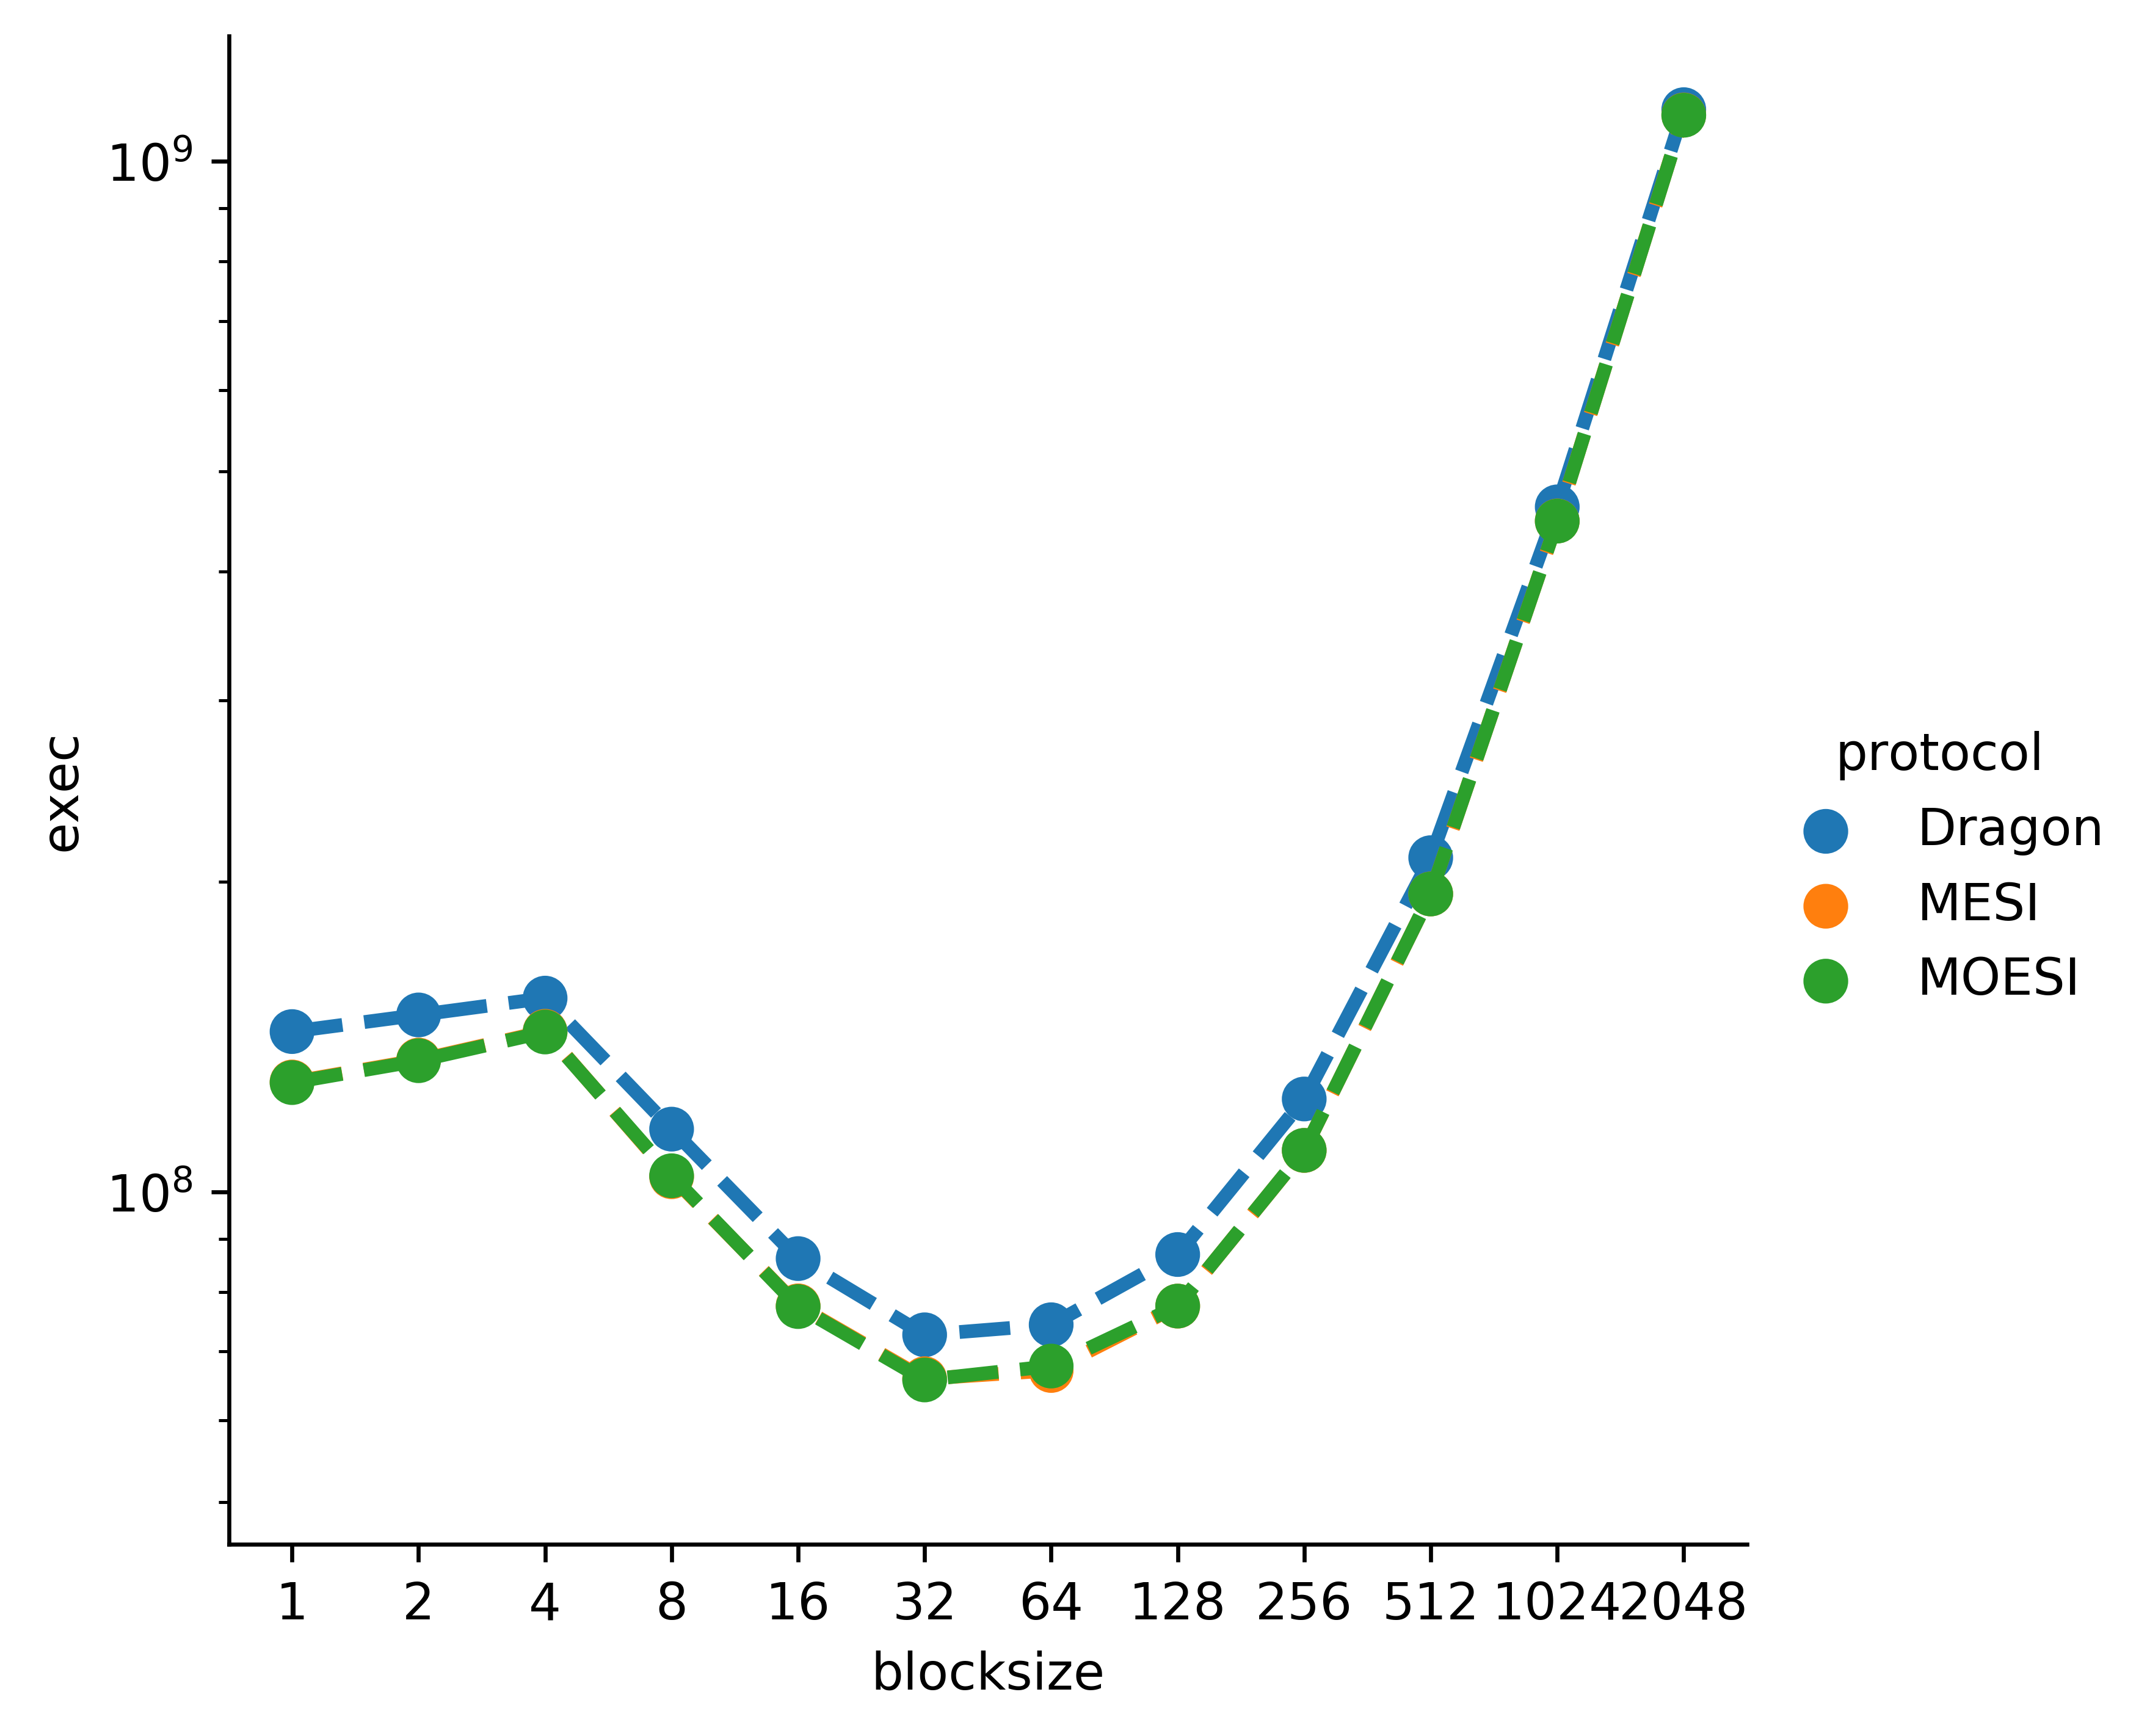
\includegraphics[width=\columnwidth]{blocksize-bodytrack}
    \caption{bodytrack}
  \end{subfigure}
  \begin{subfigure}{0.32\textwidth}
    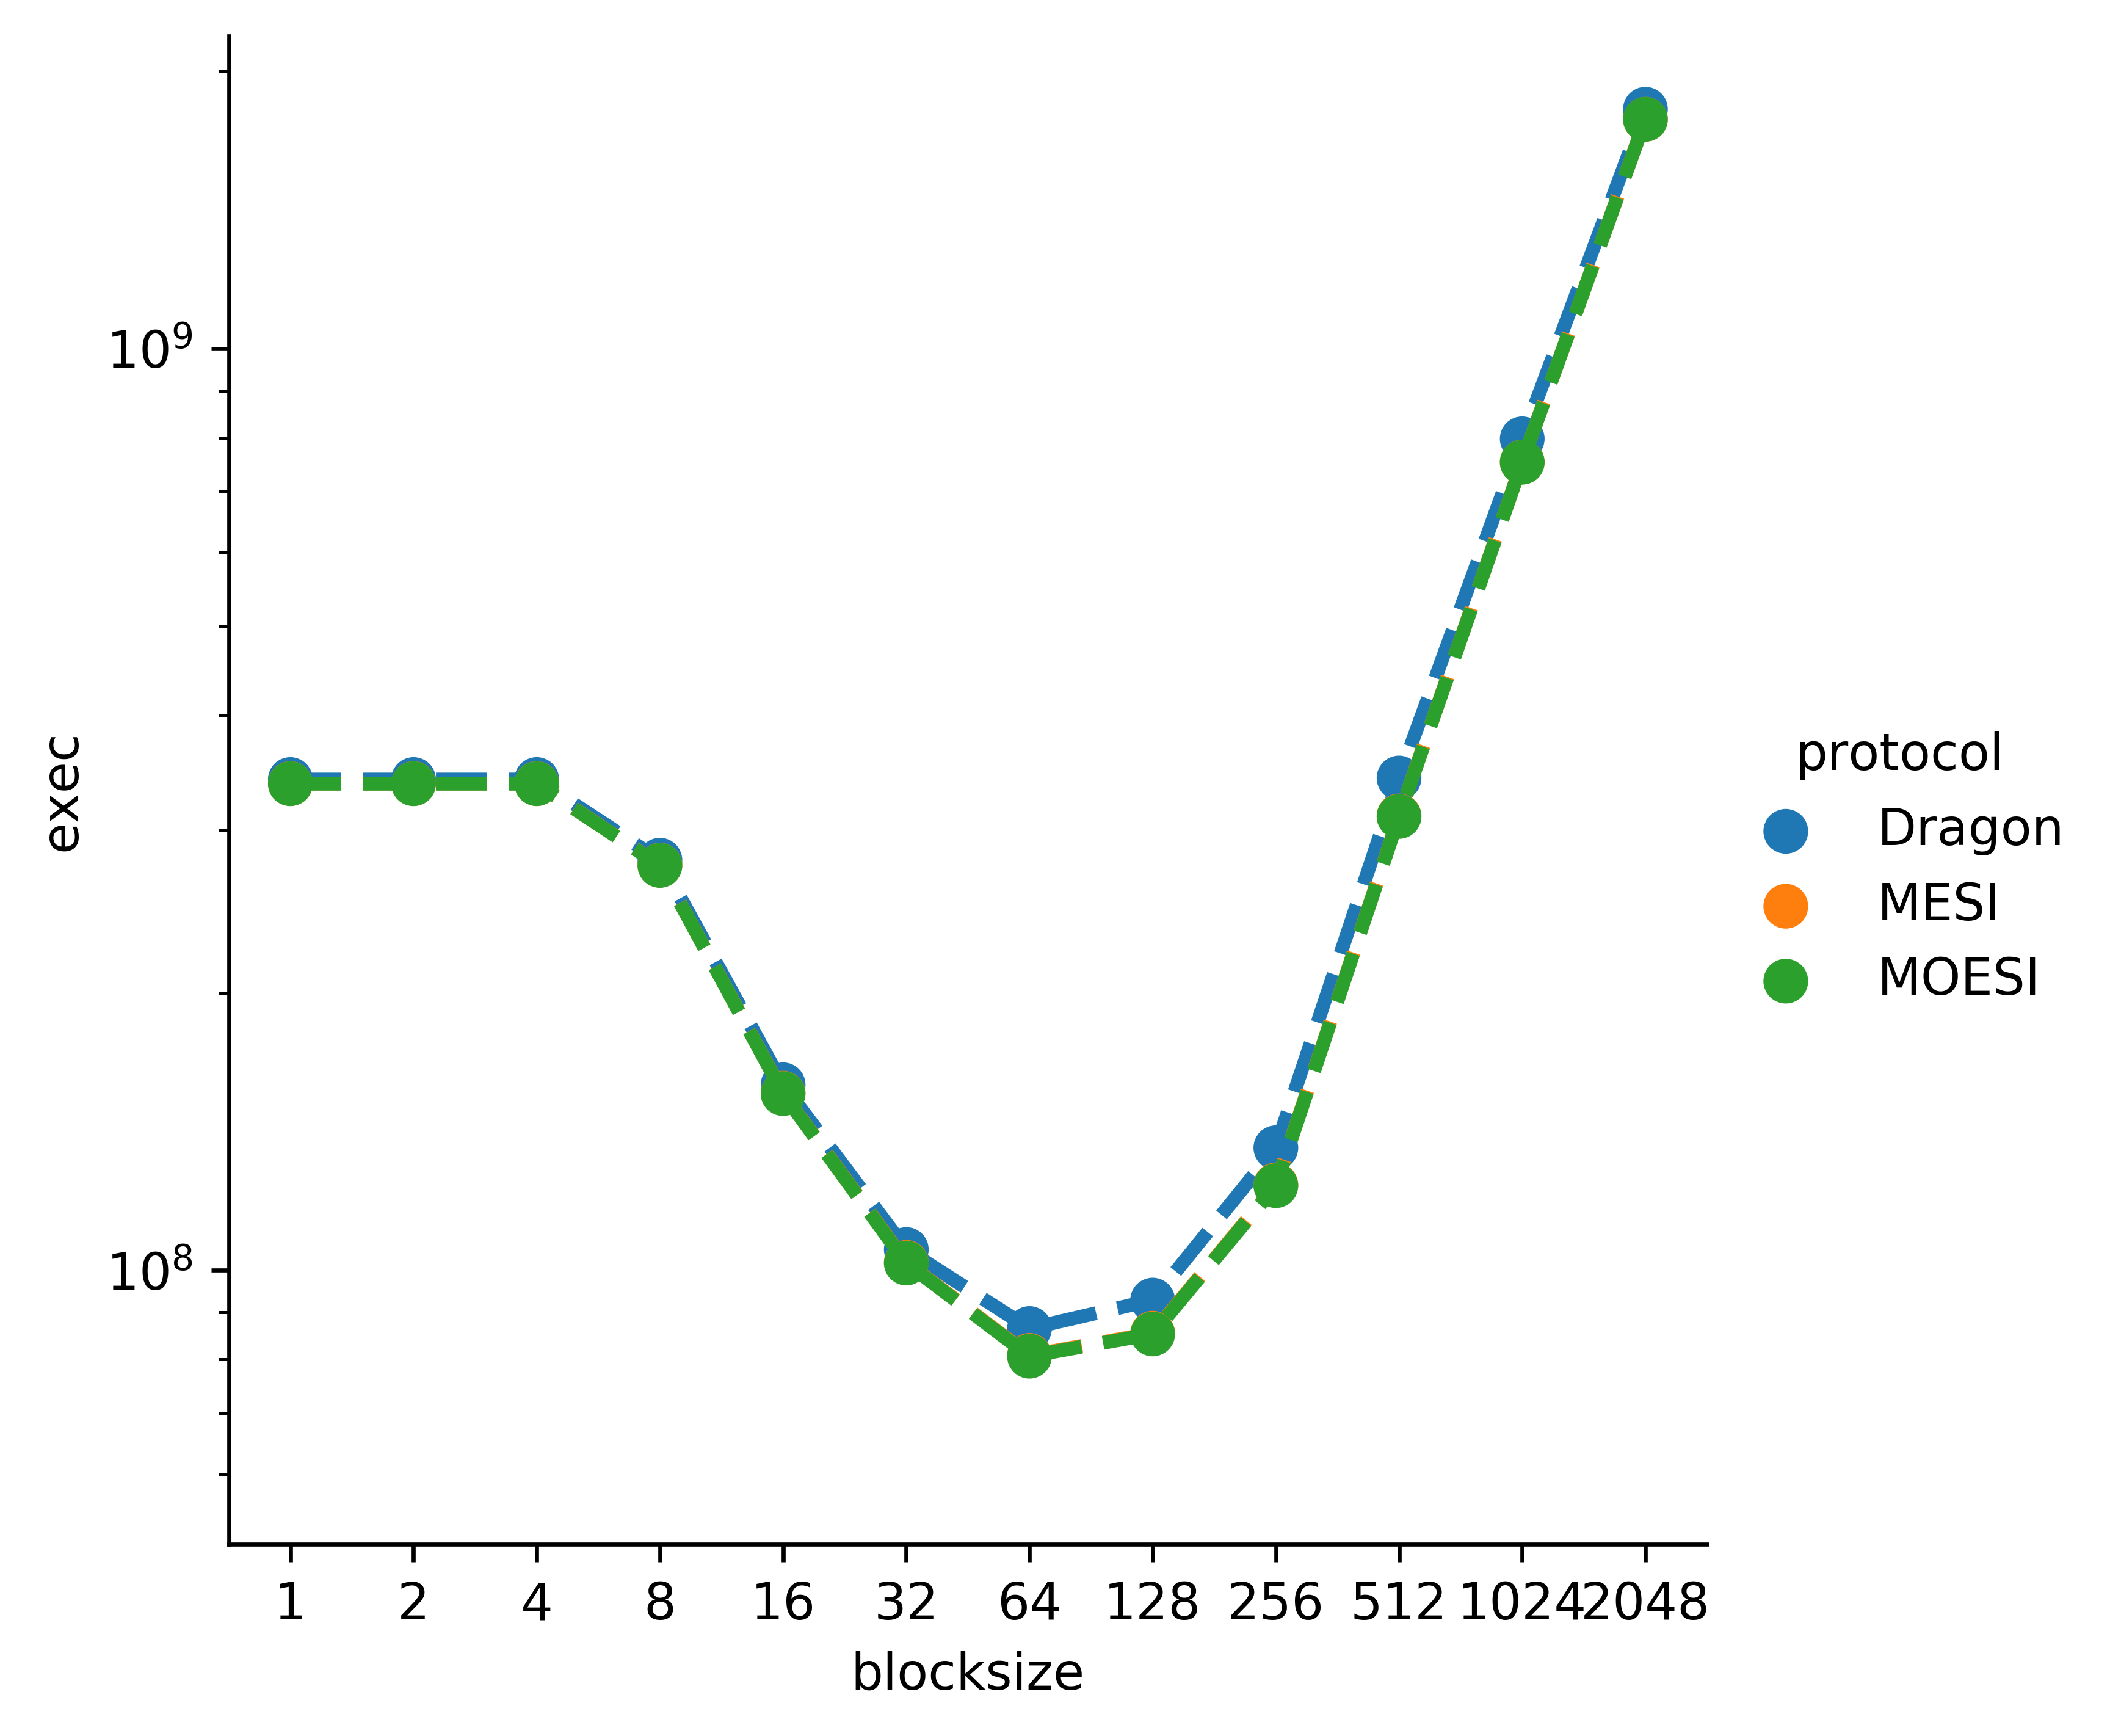
\includegraphics[width=\columnwidth]{blocksize-fluidanimate}
    \caption{fluidanimate}
  \end{subfigure}
  \caption{Plot of total execution cycles against block size with 2-way associative cache with 4 kilobytes cache size}
  \label{fig:blocksize}
\end{figure}
As seen in Figure \ref{fig:blocksize} above, the MOESI/MESI protocol once again out performs the Dragon protocol in all 3 benchmarks regardless of block size which can be attributed to the same reasons stated above. One interesting phenomenon that is observed here is how performance sharply drops past a certain block size in all 3 benchmarks. In the MOESI/MESI protocol, this is most probably due to the increased number of invalidation misses as an invalidation causes the entire cache block to be invalidated which could have contained data that would be needed in the next few instructions. In the Dragon protocol, this can be attributed to a higher overhead associated with updating the cache blocks for each write update.

\subsubsection{Associativity}
\begin{figure}[htb!]
  \centering
  \begin{subfigure}{0.32\textwidth}
    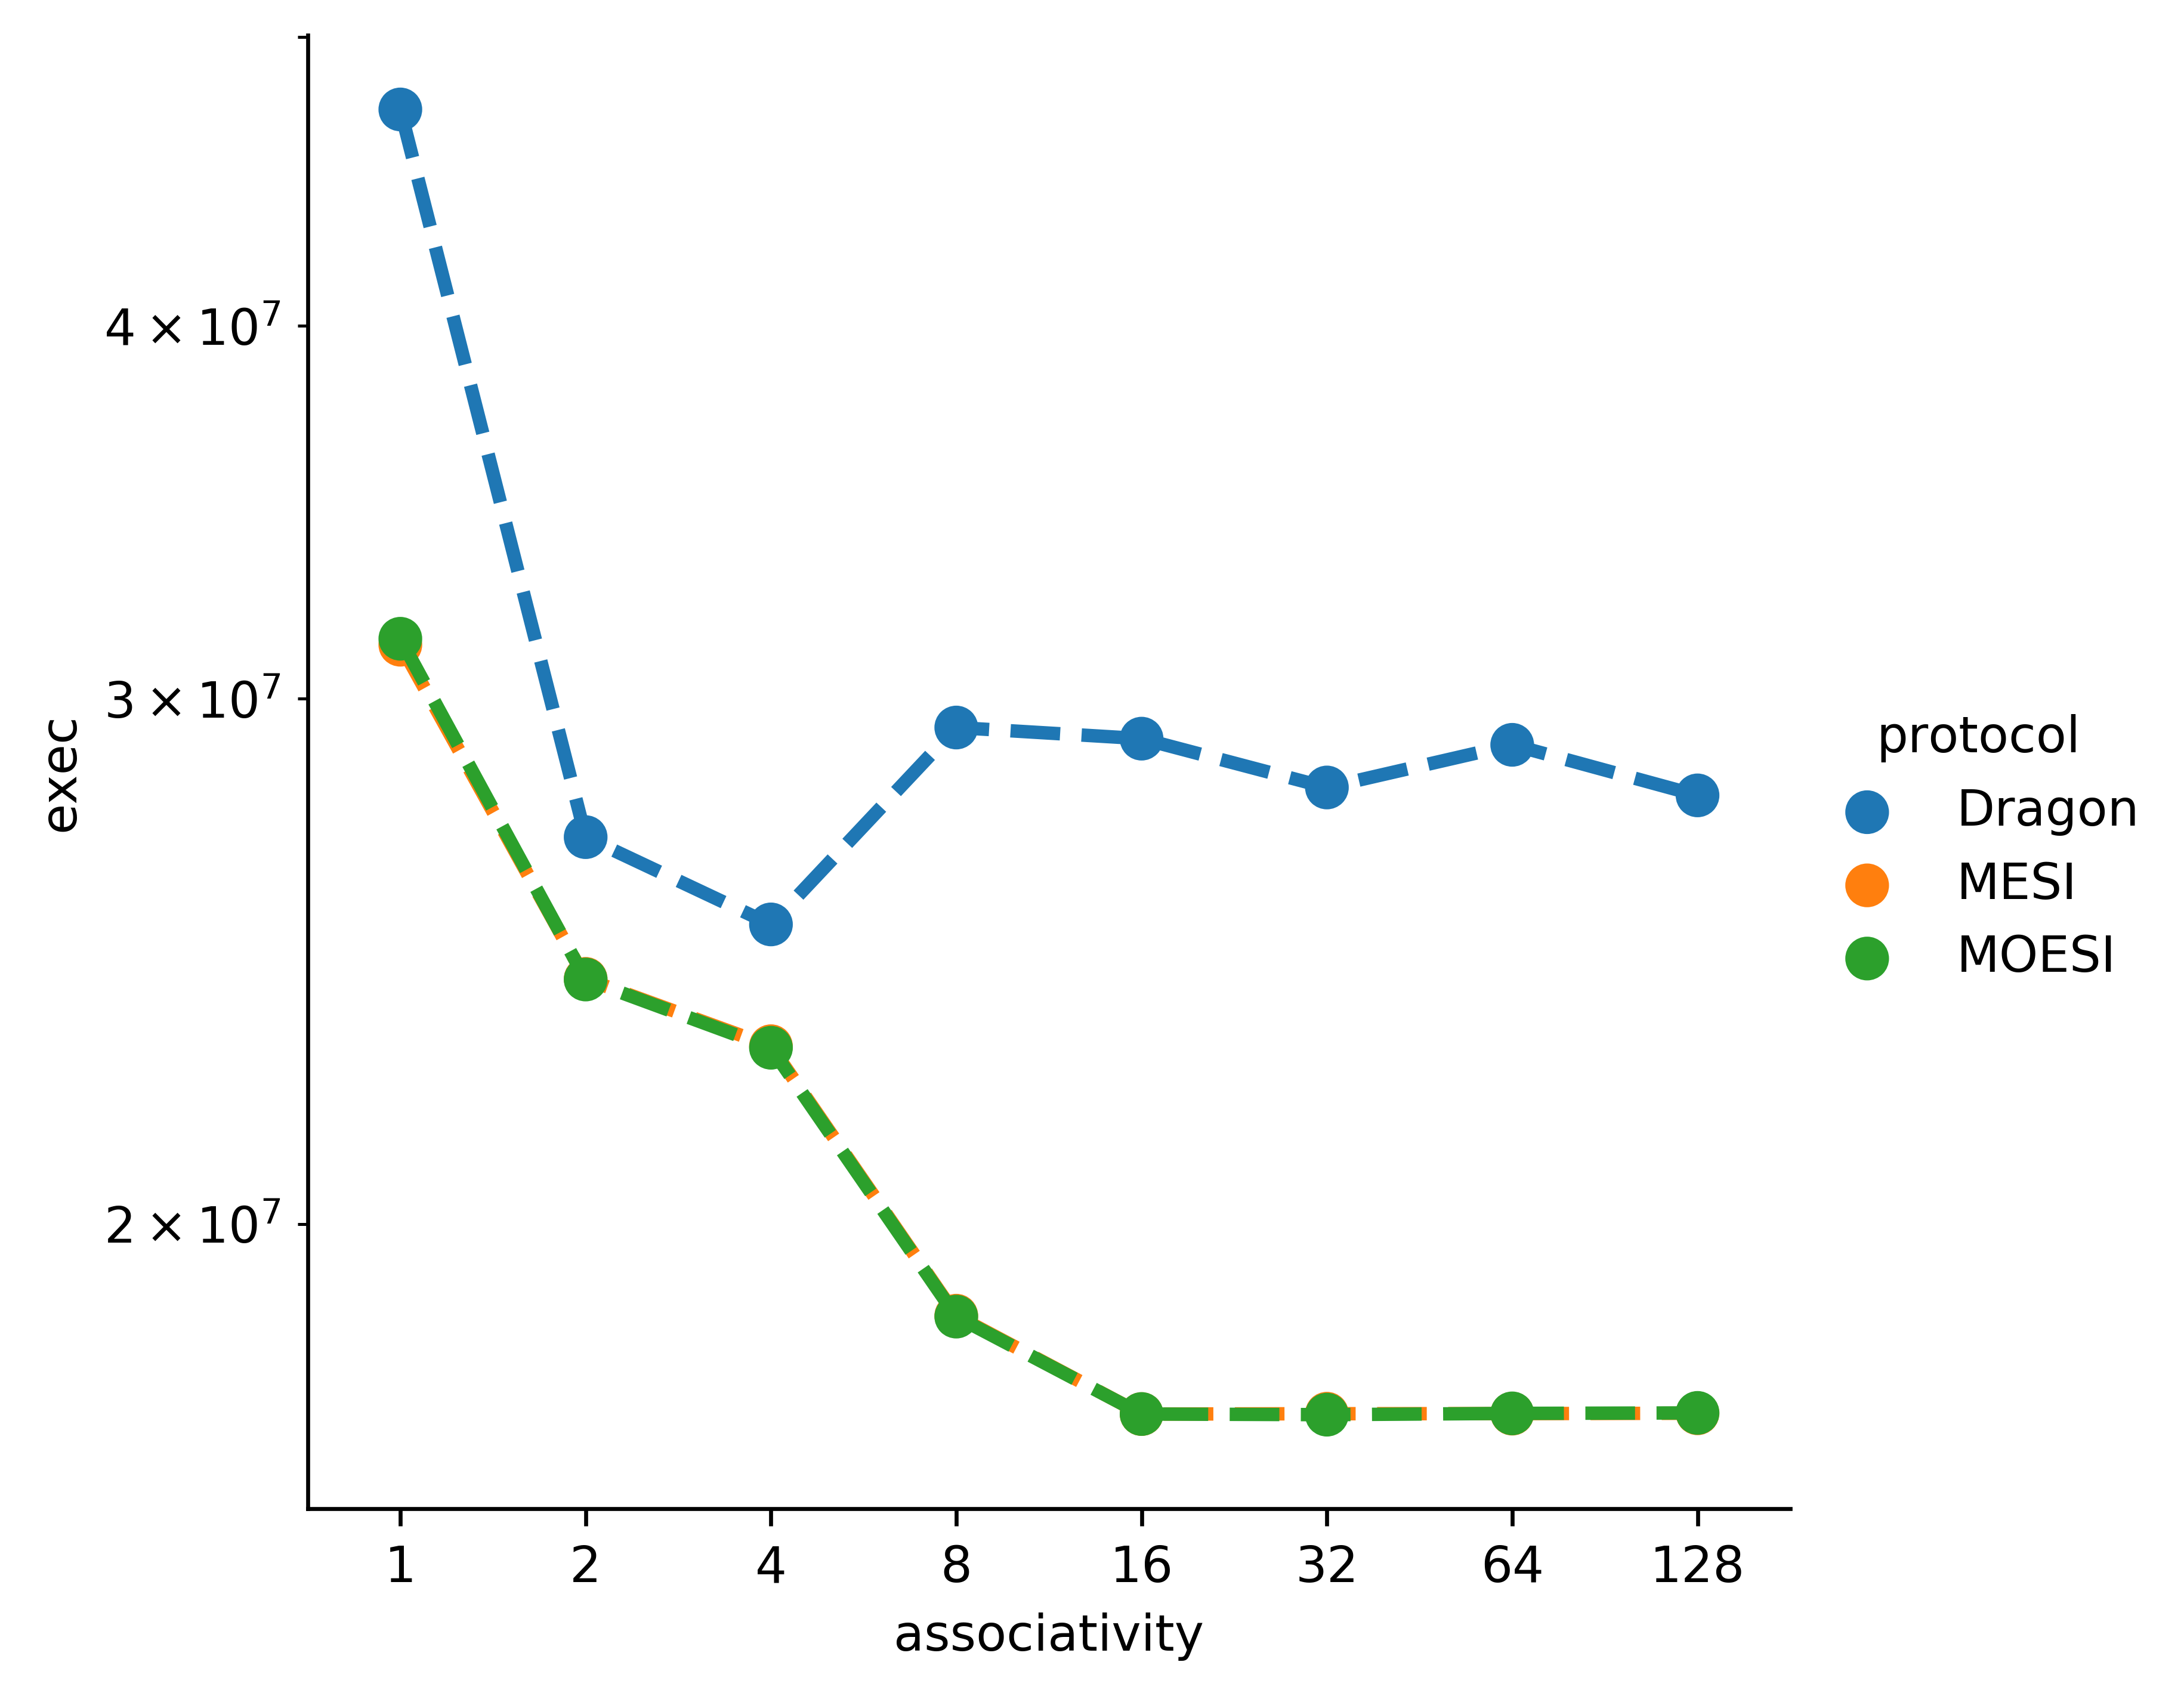
\includegraphics[width=\textwidth]{associativity-blackscholes}
    \caption{blackscholes}
  \end{subfigure}
  \begin{subfigure}{0.32\textwidth}
    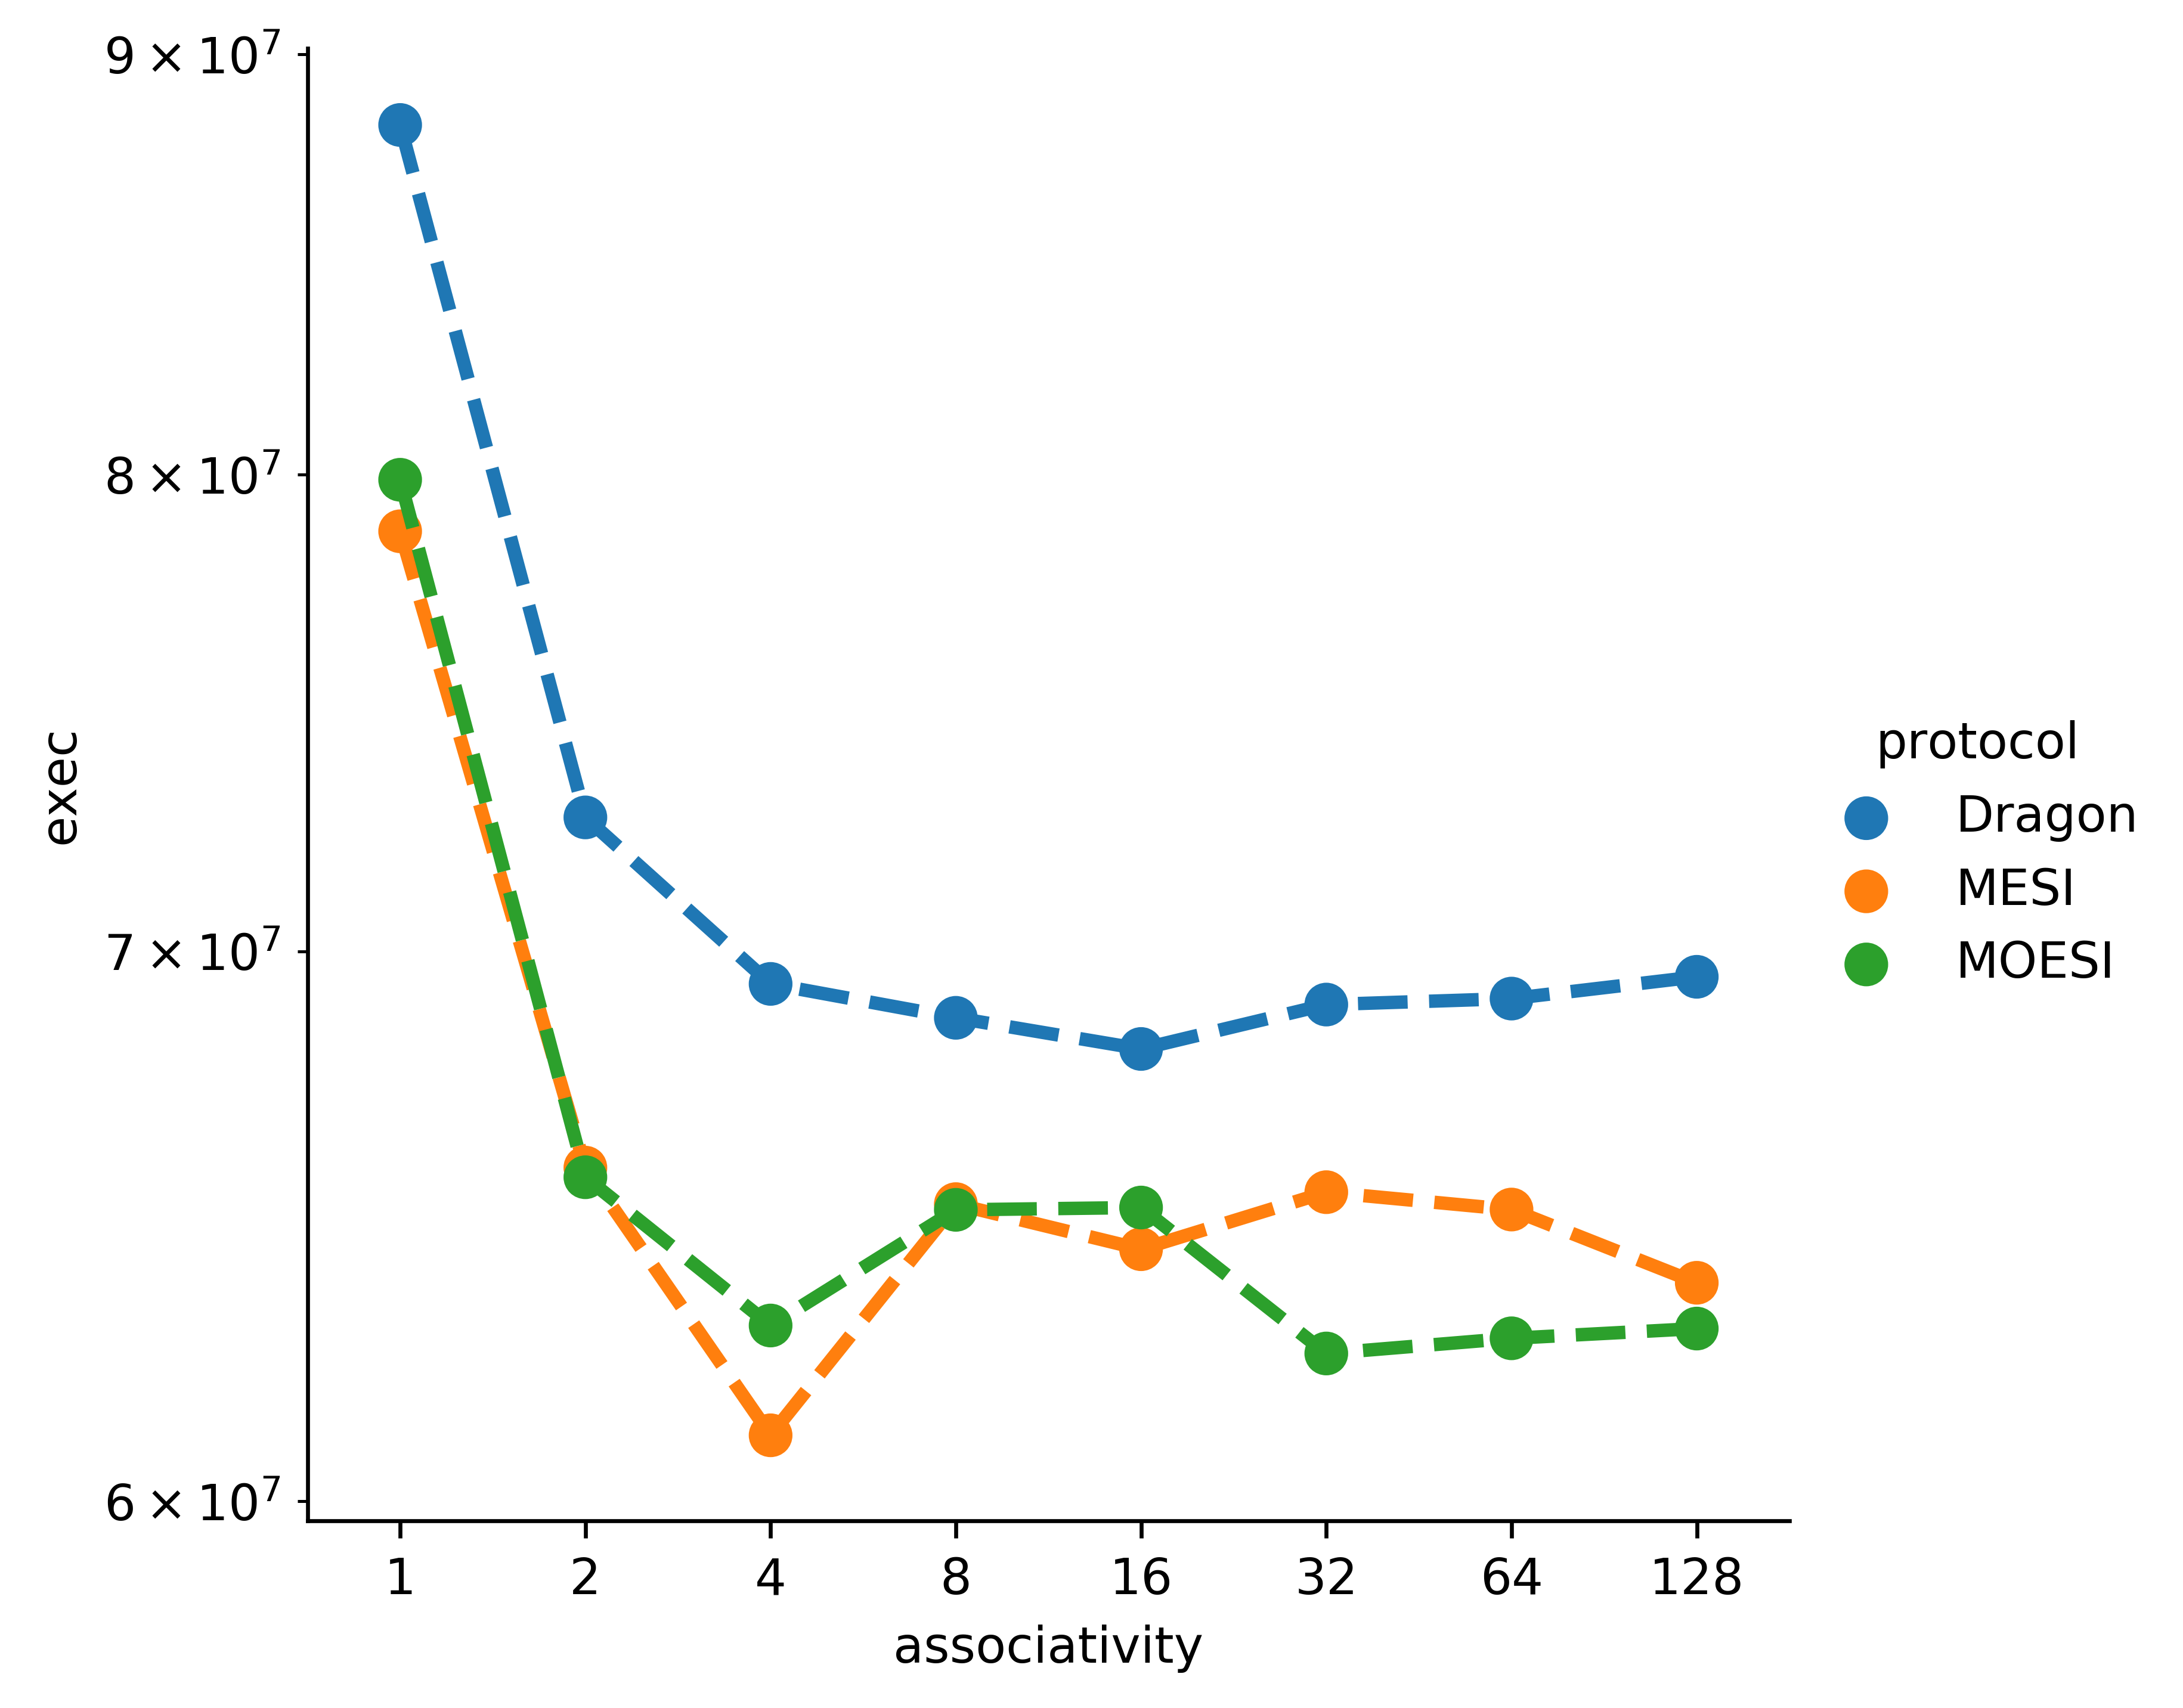
\includegraphics[width=\columnwidth]{associativity-bodytrack}
    \caption{bodytrack}
  \end{subfigure}
  \begin{subfigure}{0.32\textwidth}
    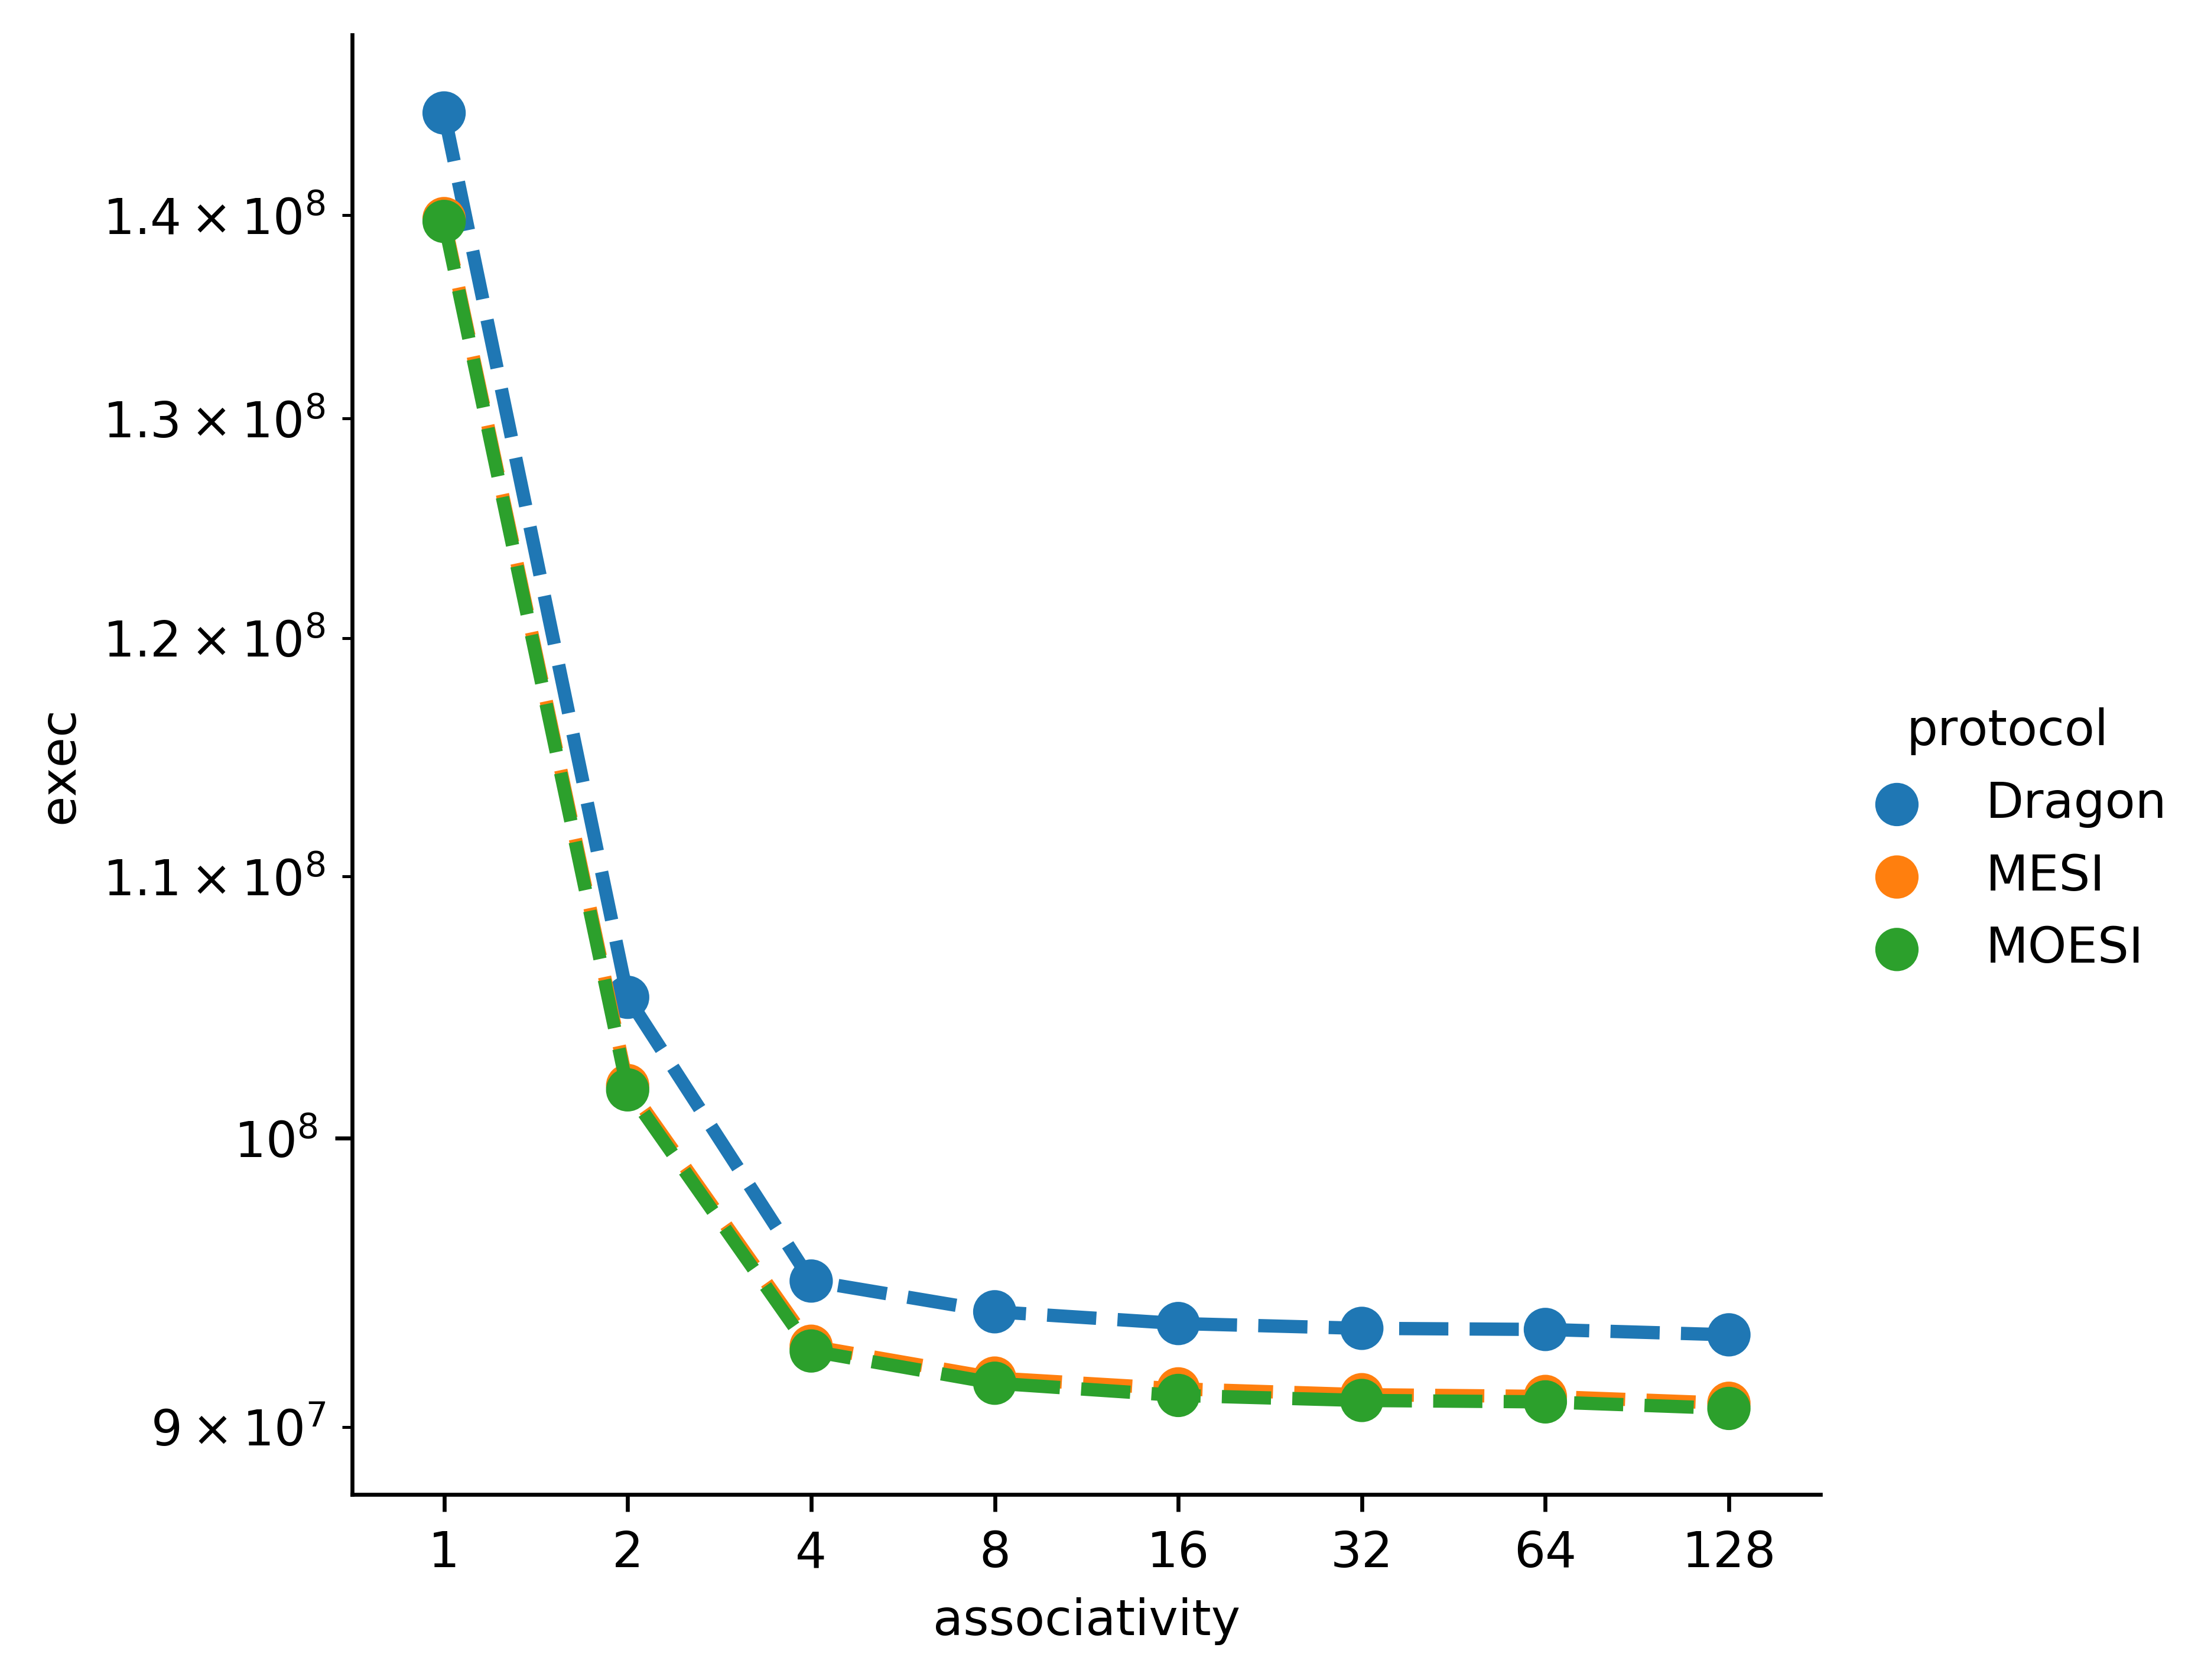
\includegraphics[width=\columnwidth]{associativity-fluidanimate}
    \caption{fluidanimate}
  \end{subfigure}
  \caption{Plot of total execution cycles against associativity with 32 bytes block size with 4 kilobytes cache size}
  \label{fig:associativity}
\end{figure}
As seen in Figure \ref{fig:associativity} above, the MOESI/MESI protocol once again out performs the Dragon protocol in all 3 benchmarks regardless of block size which can be attributed to the same reasons stated above. We can also see that the performance gained from increasing associativity flattens out in all 3 benchmarks for all the protocols. This is most likely due to the fact that the sets are not being fully utilized. More intrestingly, we can see that the performance of the MESI protocol is able to slightly beat out the performance of the MOESI protocol in the \textit{bodytrack} benchmark at some points.

\subsection{Concluding statements}
From the experiments conducted, we have shown that the MESI protocol and its variants are able to outperform the Dragon protocol across all the given benchmarks. While there are most certainly benchmarks that favour the Dragon protocol that were not tested here, these benchmarks would need to exhibit specific properties such as an interleaving of reads and writes which may not be applicable to more general applications. 

\clearpage
\bibliographystyle{ACM-Reference-Format}
\bibliography{report}
\end{document}
